%%%%%%%%%%%%%%%%%%%%%%%%%%%%%%%%%%%%%%%%%%%%%%%%%%%%%%%%%%%%%%%%%%
%%%%%%%% ICML 2016 EXAMPLE LATEX SUBMISSION FILE %%%%%%%%%%%%%%%%%
%%%%%%%%%%%%%%%%%%%%%%%%%%%%%%%%%%%%%%%%%%%%%%%%%%%%%%%%%%%%%%%%%%

% Use the following line _only_ if you're still using LaTeX 2.09.
%\documentstyle[icml2015,epsf,natbib]{article}
% If you rely on Latex2e packages, like most moden people use this:
\documentclass{article}

% use Times
\usepackage{times}
% For figures
\usepackage{graphicx} % more modern
%\usepackage{epsfig} % less modern
\usepackage{subfigure} 

% For citations
\usepackage{natbib}

% For algorithms
\usepackage{algorithm}
\usepackage{algorithmic}

% As of 2011, we use the hyperref package to produce hyperlinks in the
% resulting PDF.  If this breaks your system, please commend out the
% following usepackage line and replace \usepackage{icml2016} with
% \usepackage[nohyperref]{icml2016} above.
\usepackage{hyperref}
\hypersetup{
	colorlinks   = true, %Colours links instead of ugly boxes
	urlcolor     = blue, %Colour for external hyperlinks
	linkcolor    = blue, %Colour of internal links
	citecolor   = blue %Colour of citations
}

% Packages hyperref and algorithmic misbehave sometimes.  We can fix
% this with the following command.
\newcommand{\theHalgorithm}{\arabic{algorithm}}

% my settings
\usepackage{amssymb,amsfonts,amsmath,bbm}
\usepackage{mathrsfs}
\usepackage[all]{xy}
\usepackage{empheq}
\usepackage{algorithm,algorithmic}
\usepackage{multirow}
\usepackage{ifthen}
\usepackage[usenames]{color}
\usepackage[usenames,dvipsnames]{xcolor}
\usepackage{epstopdf}
%\usepackage{epsfig}
%\usepackage{times}
%\usepackage{helvet}
%\usepackage{courier}
%\usepackage{graphicx,subfigure}
%\usepackage{pdfpages}
%\usepackage{multirow}
%\usepackage{multicol}
\newcommand{\bbeta}{\boldsymbol{\beta}}
\newcommand{\EE}{\mathbb{E}}
\newcommand{\II}{\mathbb{I}}
\newcommand{\PP}{\mathbb{P}}
\newcommand{\RR}{\mathbb{R}}
\newcommand{\bT}{\mathbb{T}}
\newcommand{\bOne}{\mathbbm{1}}
\newcommand{\bA}{\mathbf{A}}
\newcommand{\ba}{\mathbf{a}}
\newcommand{\bB}{\mathbf{B}}
\newcommand{\bO}{\mathbf{O}}
\newcommand{\br}{\mathbf{r}}
\newcommand{\bU}{\mathbf{U}}
\newcommand{\bV}{\mathbf{V}}
\newcommand{\bw}{\mathbf{w}}
\newcommand{\bX}{\mathbf{X}}
\newcommand{\bY}{\mathbf{Y}}
\newcommand{\cA}{\mathcal{A}}
\newcommand{\cB}{\mathcal{B}}
\newcommand{\cH}{\mathcal{H}}
\newcommand{\cO}{\mathcal{O}}
\newcommand{\cS}{\mathcal{S}}
\newcommand{\argmax}{\mathrm{argmax}}
\newcommand{\trace}{\mathrm{trace}}
\newcommand{\abs}[1]{\left| #1 \right|}
\newcommand{\norm}[1]{\| #1 \|}
\newtheorem{theorem}{Theorem}[section]
\newtheorem{remark}[theorem]{Remark}
\newtheorem{proposition}[theorem]{Proposition}%[chapter]
\newtheorem{definition}[theorem]{Definition}%[chapter]
\newtheorem{corollary}[theorem]{Corollary}%[chapter]
\newtheorem{lemma}[theorem]{Lemma}%[chapter]
\newtheorem{example}[theorem]{Example}
\newenvironment{proof}{\noindent {\textbf{Proof. }}}{$\Box$ \medskip}

\newcommand{\CLemmaPrefixExi}{
	Suppose $1 = \gamma_1 \geq \gamma_2 \geq \cdots \geq \gamma_K \geq 0$. Let $A = (a_1, ..., a_{\abs{A}})$. For the time $t$ and the conjunctive objective, there exists a prefix $B$ of $A$ such that 
	$$
	p_{t, B} \geq \frac{1}{2}f_{t}^{\ast} - 1 + \gamma_{\abs{B}}, \qquad R(t, B) \geq \frac{1}{2} R(t, A).
	$$ 
}
\newcommand{\CEqDeltaEstAnd}{
	$$
	\EE_t [R(t, \bA_t) ] \leq \frac{8}{f^{\ast}} \EE_t \left[ \bbeta_{t-1}(\delta)\sum_{k=1}^{\bO_t}\norm{\gamma_k x_{t,\ba_k^t}}_{\bV_{t-1}^{-1}} \right].
	$$
}
\newcommand{\CLemmaSumXiEstimateInDet}{
  If $\lambda \geq C_\gamma$, then
  $$
    \sum_{s=1}^t \sum_{k=1}^{\bO_s} \norm{\gamma_k x_{s,\ba_{k}^s}}_{\bV_{s-1}^{-1}}^2 \leq 2\ln \left(\frac{\det(\bV_t)}{\lambda^d} \right).
  $$
}
\newcommand{\CLemmaDetVt}{
  $\det(\bV_t)$ is increasing with respect to $t$ and 
  $$
    \det(\bV_t) \leq (\lambda + C_\gamma t/d)^d.
  $$
}


\newcommand{\hidetext}[1]{}

\newcommand{\compilehidecomments}{false}

% Macro for comments:
\ifthenelse{ \equal{\compilehidecomments}{true} }{%
	\newcommand{\wei}[1]{}
	\newcommand{\yang}[1]{}
	\newcommand{\yajun}[1]{}
}{
\newcommand{\wei}[1]{{\color{blue!50!black}  [\text{Wei:} #1]}}
\newcommand{\shuai}[1]{{\color{brown!60!black} [\text{Shuai:} #1]}}
\newcommand{\shengyu}[1]{{\color{green!50!black} [\text{Shengyu:} #1]}}
}


% Employ the following version of the ``usepackage'' statement for
% submitting the draft version of the paper for review.  This will set
% the note in the first column to ``Under review.  Do not distribute.''
%\usepackage{icml2016} 

% Employ this version of the ``usepackage'' statement after the paper has
% been accepted, when creating the final version.  This will set the
% note in the first column to ``Proceedings of the...''
\usepackage[accepted]{icml2016}


% The \icmltitle you define below is probably too long as a header.
% Therefore, a short form for the running title is supplied here:
\icmltitlerunning{Contextual Combinatorial Cascading Bandits}

\begin{document} 
	
\twocolumn[
\icmltitle{Contextual Combinatorial Cascading Bandits}
	
% It is OKAY to include author information, even for blind
% submissions: the style file will automatically remove it for you
% unless you've provided the [accepted] option to the icml2015
% package.
\icmlauthor{Your Name}{email@yourdomain.edu}
\icmladdress{Your Fantastic Institute, 314159 Pi St., Palo Alto, CA 94306 USA}
\icmlauthor{Your CoAuthor's Name}{email@coauthordomain.edu}
\icmladdress{Their Fantastic Institute, 27182 Exp St., Toronto, ON M6H 2T1 CANADA}
	
% You may provide any keywords that you 
% find helpful for describing your paper; these are used to populate 
% the "keywords" metadata in the PDF but will not be shown in the document
\icmlkeywords{boring formatting information, machine learning, ICML}
	
\vskip 0.3in
]
	
\begin{abstract} 
	
We propose the {\it contextual combinatorial cascading bandits}, an online partial monitoring game where at each time step a learning agent is given a set of context information, then recommends a list of items, and observes weights from the first item until some problem-specific stopping criterion happens. In recommendation, the stopping criterion might be the first item a user selects; in network, the stopping criterion might be the first edge being blocked in a path. We also consider position discounts in the list order, which means in recommendation the agent will receive discounted reward if the user does not select the first item. We propose a UCB-type algorithm to solve our problem, C$^3$-UCB, and prove an $n$-step regret bound $\tilde{O}(\sqrt{n})$ in both the general setting and two special cases. Our work generalizes existing works and also addresses several challenges in our setting, a non-linear reward function with position discounts, contextual information and partial observability. The experiments on synthetic and real data demonstrate the advantage to involve contextual information and position discounts.

\end{abstract} 
	
\section{Introduction}

Multi-armed bandit (MAB) has been extensively studied in statistics and machine learning. The problem can be formulated as a system of $K$ base arms whose rewards are random samples from unknown distributions with unknown means. The learning agent pulls one arm every time and tries to make the cumulative regret, the expected reward difference from the best arm with highest mean, as small as possible. The problem of MAB has to deal with the trade-off between exploitation (pull the best empirical arm) and exploration (try other arms which are not sufficiently estimated).

Recently, stochastic combinatorial bandit started to draw attention \cite{gai2012combinatorial,chen2013combinatorial}. At every time step, a learning agent chooses a subset of ground items (super arm) under certain combinatorial constraints. There are several different kinds of feedback: (1) bandit feedback, where the learning agent can only obtain the reward of chosen super arm; (2) semi-bandit feedback, where the learning agent can not only obtain the reward of the chosen super arm but also the weights (or rewards) of all base arms constituting the chosen super arm; (3) cascading feedback, where the learning agent can obtain the reward of the chosen super arm and the weights of some base arms in the chosen super arm, according to some problem-specific stopping criterion for observation.

For recommendations, the cascade model is usually adopted to describe certain user behaviors. When recommended with a ordered list of items, such as web pages or advertisements, the user checks from the first item until she finds an attractive item and selects it. The items before the selected one are not attractive and the items after the selected one are unobserved. Also in networking routing problem, to determine whether a path is blocked, we check from the source node until we meet a blocked edge. The edges before the blocked one are unblocked and the edges after the blocked one are unobserved. In both of the two applications, we observe the feedbacks of a prefix of items in the chosen ordered list. The bandit problem with cascading feedback has been studied in \cite{kveton2015cascading,kveton2015combinatorial}.

Personalized recommendation is a key feature of online recommendations to improve user satisfaction by providing attractive contents to meet specific user's need. Personalization includes storing user features and historical information, managing content set, analysis of user behaviors and providing suitable content to the user. Usually, both users and contents are represented by feature vectors. User features may contain basic attributes, like age, gender and nationality, and historical behaviors. Content features may contain categories and descriptive information. Because the views of different users on the same content can vary significantly, exploration and exploitation have to be exercised at an individual level and be able to cross different contents. When each item is represented by a feature vector that can be observed by the learning agent, the problem is known as contextual combinatorial bandit, which is developed in recommender systems and studied in \cite{qin2014contextual}.

In this paper, we propose a general framework for contextual cascading bandits encompassing the applications of recommendations and network routing problems as special cases. In addition, we take position discounts into consideration. In recommendations, different positions usually give different values. In advertisement display, there are different positions in a website, the front middle, the left/right column and the bottom, and the positions in the front middle might charge highest price. Users are most satisfied if the first returned result is what they want. We introduce the position discounts to model this variant of rewards.


Putting context, cascading and position discounts together, we develop an approach called {\it contextual combinatorial cascading bandits}. This is a general framework which can describe many applications besides the above two applications.

The main contributions of this paper can be summarized as follows: (1) we propose a general framework called contextual combinatorial cascading bandit that can address recommendation problem and network routing problem; (2) we propose $C^3$-UCB, an efficient algorithm for contextual combinatorial cascading bandit, with regret bound as $\tilde{O}(\sqrt{n})$ for $n$ rounds; (3) we evaluate this algorithm on synthetic data, recommendation data and network routing data and the results show that our algorithm is effective.

\begin{table}
	\renewcommand{\arraystretch}{1.1}
	\centering
	\begin{tabular}{|c|c|c|c|}
		\hline
		 &context &triggering &position discounts \\
		\hline
		CMAB &no &yes &no \\
		\hline
		C$^2$UCB &yes &no &no  \\
		\hline
		CombCascade	&no &yes &no  \\
		\hline
		C$^3$-UCB(our) &yes &yes &yes \\
		\hline
	\end{tabular}
	\caption{Comparisons of our setting with previous ones }
	\label{table:outline}
\end{table} 

%Stochastic online learning with combinatorial actions has been studied with semi-bandit feedback \cite{chen2013combinatorial}.

\section{Related Work}

A summarized comparison of settings is listed in Table \ref{table:outline}, which we will explain in details next. And a comparison of regret bounds by different methods will be discussed in section \ref{set:diss}.

The work of \cite{kveton2015cascading} introduced the cascading model to the multi-armed bandit framework with disjunctive objective, where the set of feasible actions form a uniform matroid, and the reward of an action is $1$ if there is at least a "good" item (with weight $1$). The combinatorial cascading bandits of \cite{kveton2015combinatorial} (refered to as 'CombCascade' in Table \ref{table:outline}) generalized the framework, where each feasible action is a subset of ground items under combinatorial constraints; it studied a problem of combinatorial bandits with conjunctive objective, where each feasible action is a chain of items, and reward is $1$ if all items are "good" (have weight $1$). Our work generalizes these model and involves both contextual information and position discounts.

The experiments of \cite{kveton2015cascading} found that recommending items in increasing order of their UCBs (meaning the items with lower preference will come first) has a better performance than in decreasing order of their UCBs; the reason might be that the user first examines the items with lower preference and the learning agent will probably collect more data. The position discounts introduced will force the recommended set in the decreasing order of UCBs. The work of \cite{combes2015learning} considered a similar recommendation model to cascading bandits with position discount but they assumed that a user is interested in a single topic. In our setting, users and items are represented by general feature vectors.

Our work considers contextual combinatorial bandits with cascading feedback and nonlinear reward. \cite{li2010contextual} studied multi-armed bandit with context information. \cite{qin2014contextual} (refered to as 'C$^2$UCB' in Table \ref{table:outline}) introduced contextual combinatorial bandit with semi-bandit feedback and nonlinear reward. Their setting is more informative than ours and we have generalized their model with the same order of regret bound.

Our problem is a combinatorial partial monitoring problem where the learning agent may observe part of chosen items. \cite{agrawal1989asymptotically,bartok2012adaptive} studied partial monitoring problems but their algorithm is inefficient in our setting. \cite{lin2014combinatorial} studied combinatorial partial monitoring problem and their feedback is a fixed (with respect to chosen action) combination of weights. If chosen action is fixed, the combination of the weights to constitute feedback is not fixed in our setting.

A newer version of \cite{chen2013combinatorial} (refered to as 'CMAB' in Table \ref{table:outline}) considered probabilistic triggering base arms in stochastic combinatorial semi-bandit. When a super arm $S$ is pulled, base arm $i$ might also be triggered with a probability $p_i^{S}$. Our method can generalize their setting with contextual information. It is hard to introduce position discounts for general combinatorial bandits except when feasible actions are lists, where items are triggered in list order. To introduce position discounts, we focus on the setting where feasible actions are lists.

% and / or case	
% \section{Problem Formulation}

% We formulate the problem of {\em contextual combinatorial cascading bandit} as follows. 
% Suppose we have a finite set  $E=\{1,...,L\}$ of $L$ \textit{ground items},  also referred to as {\em base arms}. 
% Let $\Pi^k=\{(a_1,...,a_k): a_1,...,a_k \in E, a_i \neq a_j \text{ for any } i \neq j\}$ be the set of all $k$-tuples of distinct items from $E$. 
% We call each of such tuples an {\em action} of length $k$. We will use $|A|$ to denote the length of an action $A$.
% Let $\Pi^{\leq K}= \cup_{k=1}^K \Pi^{k}$ denote the set of all actions with length at most $K$, and let $\cS \subseteq \Pi^{\leq K}$ be the set of \textit{feasible actions} with length at most $K$. 

% As a convention, we always use boldface symbols to represent random variables.

% At time $t$, feature vectors $x_{t,a} \in \RR^{d \times 1}$ with $\norm{x_{t,a}}_2 \leq 1$ for every base arm $a \in E$ are revealed to the learning agent; the feature vectors combine both the information of the user and the corresponding base arm. \shengyu{Add a standard/typical example (just one sentence) to illustrate the combination?} Then the learning agent recommends a feasible action $\bA_t=(\ba_{1}^t,...,\ba_{\abs{\bA_t}}^t) \in \cS$ to a user, where notice that the length of the action is not fixed. Starting from the first item $\ba_{1}^t$, the user checks the items $(\ba_{1}^t,...,\ba_{\abs{\bA_t}}^t)$ one by one in that order. The checking process stops if the user clicks \shengyu{selects?} on one item or has checked all items without clicking \shengyu{selecting?} anyone. We use Bernoulli random variable $\bw_{t}(a) \in \{0,1\}$ as the {\em weight} of base arm $a$ at time $t$ to indicate whether the user has clicked on $a$ or not. 

% Let $\cH_t$ denote the history before the learning agent chooses action at time $t$.
% Thus $\cH_t$ contains all information and observations at time $s < t$ and context information at time $t$. Given history $\cH_t$, we assume $\bw_{t,a}$'s are mutually independent and satisfy
% \begin{equation} % eq:expectation
%   \label{eq:expectation}
%   \EE[\bw_{t,a} | \cH_t] = \theta_{\ast}^{\top} x_{t,a},
% \end{equation}
% where $\theta_{\ast}$ is an unknown $d$-dimensional vector with the assumption that $\norm{\theta_{\ast}}_2 \leq 1$ and $0 \leq \theta_{\ast}^{\top} x_{t,a} \leq 1$ for all $t, a$. 
% We define random variable $\bO_t$ as the number of observed base arms in $\bA_t$, that is, for some $k=1,2,\ldots, \abs{\bA_t}$, 
% $$
%   \bO_t = k, \text{ if } \bw_t(\ba_j^t)=0, \forall\, j < k \text{ and } \bw_t(\ba_k^t) = 1,
% $$
% or 
% $$
%   \bO_t = \abs{\bA_t}, \text{ if }\bw_t(\ba_j^t) = 0, ~~ \forall\, j \leq \abs{\bA_t}.
% $$
% At the end of every time $t$, the agent observes the first $\bO_t$ items of $\bA_t$. We say that item $a$ is {\it observed} if $a = \ba_k^t$ for some $k \leq \bO_t$. 
% Thus, $\cH_t$ consists of $\{x_s, \bA_s = (\ba_{1}^s,...,\ba_{\abs{\bA_s}}^s), \bO_s, \bw_s(\ba_k^s),x_t \mid  k \in[\bO_s], 1 \le s<t \}$.

% The agent receives some reward if the user clicks on some item. Suppose we consider the position discount: if the user clicks on the $k$-th item, then the learning agent receives reward $0 \leq \gamma_k \leq 1$. Usually the importance of the positions is decreasing: the first position is most important. So it is a reasonable assumption that
% $$
%   1 = \gamma_1 \geq \gamma_2 \geq \cdots \geq \gamma_K \geq 0.
% $$
% At the end of time $t$, the learning agent observes $\bO_t, \bw_t(\ba_k^t), k \leq \bO_t$ and receives reward
% $$
%   \br_t = \bw_t(\ba_{\bO_t}^t) \gamma_{\bO_t} = \bigvee_{k=1}^{\abs{\bA_t}} \gamma_k \bw_t(\ba_k^t).
% $$
% where we use the notation that $\bigvee_{k=1}^n a_k = \max_{1 \leq k \leq n} a_k$. Notice that the order of $\bA_t$ affects both the feed back and the reward.

% Now let us introduce a function $f$ on $A = (a_1,...,a_{\abs{A}}) \in \cS, w = (w(1),...,w(L))$ by
% \begin{align}
%   &f : \cS \times [0,1]^E \to [0,1] \nonumber \\
%   &f(A,w) = \sum_{k = 1}^{\abs{A}} \gamma_{k} \prod_{i=1}^{k-1} (1 - w(a_i)) w(a_k).
%   \label{eq:functionf}
% \end{align}
% Then we have $\br_t = f(\bA_t, \bw_t)$ and $\EE[\br_t] = f(\bA_t, \theta_{\ast}^{\top}x_t)$ where $x_t = (x_{t,1}, \cdots, x_{t,L}) \in \RR^{d \times L}$. Let 
% \begin{align*}
%   A_t^{\ast} &= \argmax_{A\in \cS} f(A,\theta_{\ast}^{\top}x_t),\\
%   f_t^{\ast} &= f(A_t^{\ast}, \theta_{\ast}^{\top}x_t).
% \end{align*}
% The goal of our learning algorithm is to minimize the expected cumulative regret in $T$ steps
% $$
%   R(T) = \EE\left[\sum_{t=1}^T R(t, \bA_t)\right].
% $$
% where $R(t, A) = f_t^{\ast} - f(A, \theta_{\ast}^{\top}x_t)$.

% The above formulation is on the disjunctive objective, that is, at a time step the agent stops as soon as she reveals a base arm at a position $k$ in the sequence with weight $1$ and she receives reward $\gamma_k$ as the result. 
% Similarly, we could also consider the case of conjunctive objective. 
% We also use Bernoulli random variable $\bw_{t}(a) \in \{0,1\}$ to indicate the weight of item $a$ at time $t$ satisfying Equation \eqref{eq:expectation}). 
% The learning agent observes all items until the first one with weight $0$. 
% Suppose we also consider partial reward: if the $k$-th item is the first item with weight $0$, then the learning agent receives reward $\gamma_k'$; if all items have weight $1$, the learning agent receives reward $1$. 
% The more items the learning agent reveals, the more reward the agent should receive. It is reasonable to assume that
% $$
%   0 = \gamma'_1 \leq \gamma'_2 \leq \cdots \leq \gamma'_K \leq 1.
% $$
% At the end of time $t$, the learning agent observes $\bO_{\wedge, t}, \bw_t(\ba_k^t), k \leq \bO_{\wedge, t}$ and receives reward $\br_{\wedge, t}$:
% \begin{align*}
%   \br_{\wedge, t} &= \begin{cases}
%     \gamma_{\bO_{\wedge, t}}'  &\text{if } \bw_t(\ba_{\bO_{\wedge, t}}^t) = 0,\\
%     1 &\text{if } \bw_t(\ba_{\bO_{\wedge, t}}^t) = 1,
%   \end{cases}\\
%   &=\begin{cases}
%     \gamma_{k}'  &\text{if } \bw_t(\ba_{i}^t) = 1, i < k, \bw_t(\ba_{k}^t) = 0,\\
%     1 &\text{if } \bw_t(\ba_{i}^t) = 1, i\leq \abs{\bA_t}.
%   \end{cases}
% \end{align*}

% If we define a function $f_{\wedge}$ on $A = (a_1, \ldots, a_{\abs{A}}) \in \cS, w = (w(1), \ldots, w(L))$ by
% \begin{align}
%   &f_{\wedge} : \cS \times [0,1]^E \to [0,1] \nonumber \\
%   &f_{\wedge}(A,w) = \sum_{k = 1}^{\abs{A}} \gamma_k' \prod_{i = 1}^{k - 1} w(a_i)(1 - w(a_k)) + \prod_{i=1}^{\abs{A}}w(a_i),
%   \label{eq:functionfstar}
% \end{align}
% then we have $\br_{\wedge, t} = f_{\wedge}(\bA_t, \bw_t)$ and $\EE[\br_{\wedge, t}] = f_{\wedge}(\bA_t, \theta_{\ast}^{\top}x_t)$ where $x_t = (x_{t,1}, \cdots, x_{t,L}) \in \RR^{d \times L}$. To simplify notations, we assume 
% $$
%   \gamma_k' = 1 - \gamma_k.
% $$
% Then it holds that
% \begin{equation} %eq:ConDisRelation
%   \label{eq:ConDisRelation}
%   f_{\wedge}(A, w) = 1 - f(A, 1 - w).
% \end{equation}
% Let 
% \begin{align*}
%   A_{\wedge, t}^{\ast} &= \argmax_{A\in \cS} f(A,\theta_{\ast}^{\top}x_t),\\
%   f_{\wedge, t}^{\ast} &= f(A_t^{\ast}, \theta_{\ast}^{\top}x_t).
% \end{align*}
% For the conjunctive objective, the goal of our learning algorithm is to minimize the expected cumulative regret in $T$ steps
% $$
%   R_{\wedge}(T) = \EE\left[\sum_{t=1}^T R_{\wedge}(t, \bA_t)\right].
% $$
% where $R_{\wedge}(t, A) = f_{\wedge, t}^{\ast} - f_{\wedge}(A, \theta_{\ast}^{\top}x_t)$.

\section{Problem Formulation}

We formulate the problem of {\em contextual combinatorial cascading bandits} as follows. Suppose we have a finite set $E=\{1,...,L\}$ of $L$ \textit{ground items}, also referred to as {\em base arms}. Let $\Pi^k=\{(a_1,...,a_k): a_1,...,a_k \in E, a_i \neq a_j \text{ for any } i \neq j\}$ be the set of all $k$-tuples of distinct items from $E$; we call each of such tuples an {\em action} of length $k$. We will use $|A|$ to denote the length of an action $A$. Let $\Pi^{\leq K}= \cup_{k=1}^K \Pi^{k}$ denote the set of all actions with length at most $K$, and let $\cS \subseteq \Pi^{\leq K}$ be the set of \textit{feasible actions} with length at most $K$.

As a convention, we always use boldface symbols to represent random variables.

At time $t$, feature vectors $x_{t,a} \in \RR^{d \times 1}$ with $\norm{x_{t,a}}_2 \leq 1$ for every base arm $a \in E$ are revealed to the learning agent; the feature vectors combine both the information of the user and the corresponding base arm. For example, suppose the user at time $t$ is represented by the feature vector $u_t$ and the feature vector of the base arm $a$ is $v_a$, then we can let $x_{t,a} = (u_t, v_a)$ be the combined feature vector of base arm $a$ at time $t$. Then the learning agent recommends a feasible action $\bA_t=\{ \ba_{1}^t,...,\ba_{\abs{\bA_t}}^t \} \in \cS$ to the user. Next according to the user behaviors under the stopping criterion, we observe the weights of fist $\bO_t$ base arms in $\bA_t$, which are $\bw_t(\ba_k^t), k \leq \bO_t$. For example in recommender systems, the stopping criterion might be that the user has found an attractive item or has checked all items.

Let $\cH_t$ denote the history before the learning agent chooses action at time $t$. Thus $\cH_t$ contains all information including observations at time $s < t$ and context information at time $t$. Given history $\cH_t$, we assume $\bw_{t,a}$'s are mutually independent random variables with sub-Gaussian tails and satisfy
\begin{equation} % eq:expectation
  \label{eq:expectation}
  \EE[\bw_{t,a} | \cH_t] = \theta_{\ast}^{\top} x_{t,a},
\end{equation}
where $\theta_{\ast}$ is an unknown $d$-dimensional vector with the assumption that $\norm{\theta_{\ast}}_2 \leq 1$ and $0 \leq \theta_{\ast}^{\top} x_{t,a} \leq 1$ for all $t, a$. Following standard assumptions of stochastic MABs, a reward distribution has R-sub-Gaussian tail if for some known constant $R > 0$ and all $\lambda \in \RR$, 
$$
\EE[\exp(\lambda(\bw_{t,a} - \theta_{\ast}^{\top} x_{t,a})) | \cH_t] \leq \exp(\lambda^2 R^2 / 2).
$$
Define $w_{t,a} = \theta_{\ast}^{\top} x_{t,a}$ as the expected weight of base arm $a$ at time $t$. 

We define random variable $\bO_t$ as the number of observed base arms in $\bA_t$. At the end of every time $t$, the agent observes the first $\bO_t$ items of $\bA_t$. We say that item $a$ is {\it observed} if $a = \ba_k^t$ for some $k \leq \bO_t$. Thus, $\cH_t$ consists of $\{x_s, \bA_s = (\ba_{1}^s,...,\ba_{\abs{\bA_s}}^s), \bO_s, \bw_s(\ba_k^s) \}_{k\leq \bO_s, s\leq t}$ and $\{x_t\}$, where $x_s = (x_{s,a})_{a \in E}$ denotes all context information at time $s$.

We introduce position discounts $\gamma_k \in [0,1], k\leq K$. For example in website recommendations, if the user selects the first website, the learning agent will receive reward $1$; and if the user selects the $k$-th website, the learning agent will receive reward $\gamma_k$.

The reward function on round $t$ is an application dependent function. We assume the expected reward function of action $A$ is a function of expected weights $w$, denoted by $f(A,w)$, and satisfies the following two assumptions.

\paragraph{Monotonicity}
The expected reward function $f(A, w)$ is a non-decreasing with respect to $w$. For any $w,w'\in \RR^E$, if $w(i) \leq w'(i)$, we have $f(A, w) \leq f(A, w')$.

\paragraph{Lipschitz continuity}
The expected reward function $f(A, w)$ is a Lipschitz continuous with respect to $w$ together with position discount parameters $\gamma_k, k\leq K$. In particular, there is a constant $B>0$ such that, for any $w,w'$, we have
$$
	|f(A, w) - f(A, w')| \leq B \sum_{k=1}^{|A|} \gamma_k |w(a_k) - w'(a_k)|,
$$
where $A = (a_1, \ldots, a_{|A|})$.

The assumption of Lipschitz continuity gives an estimate of changes in reward function. To obtain a good estimation of reward function, the position $k$ with large discount number $\gamma_k$ need a good estimation of $w(a_k)$. This means the positions with large discount numbers are more important to the reward function, or the reward function is more sensitive to these positions. For example in website recommendations, the learning agent will receive highest reward if the user selects the first item, so the first position is most important. 

Notice that we don't require the knowledge how $f(A, w)$ is defined. We only assume the agent has access to an oracle $\cO_{\cS}(w)$. More precisely, an oracle $\cO_{\cS}(w)$ is  called an $\alpha$-approximation oracle for some $\alpha \leq 1$, if given input $w$, the oracle always returns an action $A = \cO_{\cS}(w) \in \cS$ satisfying $f(A,w) \geq \alpha f(A^*,w)$ where $A^* = \argmax_{A\in\cS} f(A, w)$.

The $\alpha$-regret of action $A$ on time $t$ can be written as
$$
R(t, A) = \alpha f_t^{\ast} - f(A, w_t),
$$
where $f_t^{\ast} = f(A_t^*, w_t)$ and $A_t^* = \argmax_{A\in\cS} f(A, w_t)$. Our goal is to minimize the cumulative regret $R(n) = \sum_{t=1}^n R(t, \bA_t)$.

\section{Algorithms and Results}

\subsection{Algorithm}

\begin{algorithm} %C^3-UCB algorithm
	\caption{C$^3$-UCB}
	\label{alg:ConComCascade}
	\begin{algorithmic}[1]
		\STATE {Parameters:}
		\STATE {\qquad $\gamma_k\in[0,1], k \leq K; \delta > 0; \lambda \geq C_\gamma = \sum_{k=1}^{K} \gamma_k^2$}
		\STATE {Initialization:}
		\STATE {\qquad $\hat{\theta}_0 = 0, \bbeta_0(\delta) = 1, \bV_0 = \lambda I, \bX_0=\emptyset, \bY_0=\emptyset$}
		
		\FORALL {$t=1,2,\ldots$}
		\STATE {Obtain context $x_{t,a}$ for all $a\in E$}
		\STATE {$\forall a\in E$, compute}
		\STATE {~~ $\bU_t(a) = \min\{\hat{\theta}_{t-1}^{\top}x_{t,a} + \bbeta_{t-1}(\delta)\norm{x_{t,a}}_{\bV_{t-1}^{-1}}, 1\}$} 
		
		\STATE {//Choose action $\bA_t$ using UCBs $\bU_t$}
		\STATE { $\bA_t=(\ba_1^t,...,\ba_{\abs{\bA_t}}^t) \leftarrow \cO_{\cS}(\bU_t)$ } 
		\STATE {Play $\bA_t$ and observe $\bO_t, \bw_t(\ba_k^t), k\in[\bO_t]$}
		
		\STATE {//Update statistics}
		\STATE {$\bV_{t} \leftarrow \bV_{t-1} + \sum_{k=1}^{\bO_t} \gamma_k^2 x_{t, \ba_k^t}x_{t, \ba_k^t}^{\top}$}
		\STATE {$\bX_t \leftarrow [\bX_{t-1}; ~\gamma_1 x_{t, \ba_1^t}^{\top};  ~\ldots; ~\gamma_{\bO_t} x_{t, \ba_{\bO_t}^t}^{\top}]$}
		\STATE {$\bY_t \leftarrow [\bY_{t-1}; ~\gamma_1 \bw(\ba_1^t); ~\ldots; ~\gamma_{\bO_t} \bw_t(\ba_{\bO_t}^t)]$}
		\STATE {$\hat{\theta}_t \leftarrow (\bX_t^\top \bX_t + \lambda I)^{-1} \bX_{t}^\top \bY_t$}
		\STATE {$\bbeta_{t}(\delta) \leftarrow R \sqrt{\ln(\det(\bV_{t})/(\lambda^d \delta^2))} + \sqrt{\lambda}$ }
		\ENDFOR {~~$t$}
	\end{algorithmic}
\end{algorithm}

At time $t$, we denote $\EE_t[\cdot] = \EE[\cdot | \cH_t]$, where $\cH_t$ is the history a time $t$ before the learning agent chooses her action. By Equation \eqref{eq:expectation}, we have 
$$
  \EE[(\gamma_k \bw_{s,\ba_k^s}) | \cH_{s}] = \theta_*^{\top} (\gamma_k x_{s,\ba_k^s}).
$$
Using the ridge regression of data 
$$
  \{(\gamma_k x_{s,\ba_k^s}, \gamma_k \bw_{s,\ba_k^s})\}_{k \in[\bO_s], s\in[t]},
$$
we get an $l^2$-regularized least-squares estimate of $\theta_*$ with regularization parameter $\lambda > 0$:
\begin{equation}
  \hat{\theta}_t = (\bX_t^{\top}\bX_t + \lambda I)^{-1} \bX_t^{\top} \bY_t,
\end{equation}
where $\bX_t \in \RR^{(\sum_{s=1}^{t}\bO_s) \times d}$ is the matrix whose rows are $\gamma_k x_{s,\ba_k^s}^{\top}$ and $\bY_t$ is the column vector whose elements are $\gamma_k \bw_s(\ba_k^s)$, $k \in[\bO_s], s\in[t]$. Let
$$
  \bV_t = \bX_t^{\top} \bX_t + \lambda I = \lambda I + \sum_{s=1}^{t} \sum_{k=1}^{\bO_s} \gamma_k^2 x_{s,\ba_k^s}x_{s,\ba_k^s}^{\top}.
$$
Then $\bV_t \in \RR^{d \times d}$ is a symmetric positive definite matrix. For any symmetric positive definite matrix $V \in \RR^{d \times d} $ and any vector $x \in \RR^{d \times 1}$, we define the $2$-norm of $x$ based on $V$ to be $\norm{x}_V = (x^{\top} V x)^{\frac{1}{2}}$. Next we build on a good estimate of the difference between $\hat{\theta}_t$ and $\theta_*$ by Theorem 2 in \cite{abbasi2011improved}, which states the following results.

\begin{lemma} $\mathrm{\cite{abbasi2011improved}}$ %estimate of theta
  \label{thm:theta_estimate}
  Let 
  \begin{equation}
    \bbeta_{t}(\delta) = R\sqrt{\ln\left(\frac{\det(\bV_{t})}{\lambda^d \delta^2}\right)} + \sqrt{\lambda}. \label{eq:definebeta}
  \end{equation}
  Then for any $\delta > 0$, with probability at least $1 - \delta$, for all $t > 0$, we have
  \begin{equation}
    \label{eq:estimateTheta}
    \norm{\hat{\theta}_t - \theta_{\ast}}_{\bV_{t}} \leq \bbeta_{t}(\delta).
  \end{equation}
\end{lemma}

This theorem states that with high probability, the estimate $\hat{\theta}$ lies in the ellipsoid centered at $\theta_*$ with confidence radius $\bbeta_t(\delta)$ under $\bV_t$ norm. 
Building on this, we can define an upper confidence bound of the expected weight of base arm $a$ by
\begin{equation}
  \label{eq:defU}
  \bU_t(a) = \min\left\{\hat{\theta}_{t-1}^{\top}x_{t,a} + \bbeta_{t-1}(\delta)\norm{x_{t,a}}_{\bV_{t-1}^{-1}}, 1 \right\}.
\end{equation}

The fact that $\bU_t(a)$ is an upper confidence bound of expected weight $w_{t, a} = \theta_*^{\top} x_{t,a}$ is proved in the following lemma.
\begin{lemma} %estimate of U
  \label{lem:estimateU}
  When Eq.\eqref{eq:estimateTheta} holds for time $t-1$, we have
  $$
    0 \leq \bU_t(a) - w_{t,a} \leq 2 \bbeta_{t-1}(\delta)\norm{x_{t,a}}_{\bV_{t-1}^{-1}}.
  $$
\end{lemma}
\begin{proof}
	$w_{t,a} = \theta_*^{\top} x_{t,a}$. By Holder's inequality,
	\begin{align*}
		\abs{\hat{\theta}_{t-1}^{\top}x_{t,a} - \theta_{\ast}^{\top}x_{t,a}} &\leq \norm{\hat{\theta}_{t-1} - \theta_{\ast}}_{\bV_{t-1}} \norm{x_{t,a}}_{\bV_{t-1}^{-1}} \\
		&\leq \bbeta_{t-1}(\delta)\norm{x_{t,a}}_{\bV_{t-1}^{-1}}.
	\end{align*}
	Then because
	\begin{align*}
		0 &\leq (\hat{\theta}_{t-1}^{\top}x_{t,a} + \bbeta_{t-1}(\delta)\norm{x_{t,a}}_{\bV_{t-1}^{-1}}) - \theta_{\ast}^{\top}x_{t,a} \\
		&\leq 2 \bbeta_{t-1}(\delta)\norm{x_{t,a}}_{\bV_{t-1}^{-1}}
	\end{align*}
	and the definition of $\bU_t$ in \ref{lem:estimateU}, we can obtain the result.
\end{proof}

Our proposed algorithm, C$^3$-UCB, is described in Algorithm \ref{alg:ConComCascade}. First, the learning agent computes the upper confidence bounds (UCBs) $\bU_t \in [0,1]^{E}$ for the expected weights of all base arms in $E$. Second, the agent uses the computed UCBs, $\bU_t$, to select an action $\bA_t = \{\ba_{1}^t,..., \ba_{\abs{\bA_t}}^t \}$. Third, the user checks from the first base arm in $\bA_t$ and stops after checking the $\bO_t$-th base arm and the agents observes $\bw_t(\ba_k^t), k\leq \bO_t$. Then, the learning agent updates $\bV_t, \bX_t, \bY_t$ in order to get a newer estimate $\hat{\theta}_t$ of $\theta_*$ and new confidence radius $\bbeta_t(\delta)$. In this part, we use the notation $[A; B]$ to denote the matrix obtained by stacking A and B vertically like $\begin{pmatrix} A\\ B\end{pmatrix}$.

\subsection{Results}

\subsubsection{General Results}

To state our main theorem, we need some definitions. Let $p_{t, A}$ be the {\em probability of full observation of $A$}, that is the probability of observing all base arms of $A = (a_1, \ldots, a_{\abs{A}})$ at time $t$. Let $p^* = \min_{1 \leq t \leq T} \min_{A \in \cS} ~ p_{t, A}$ to be the minimal probability that an action could have all base arms observed over all time. The following is the main theorem on the regret achieved by our C$^3$-UCB algorithm.

\begin{theorem} %main theorem
	\label{thm:main}
	Suppose the expected reward function $f(A, w)$ is a function of expected weights and satisfies the requirements of monotonicity and Lipschitz continuity. Assume there is an $\alpha$-approximation oracle $\cO_{\cS}$. Then for any $\delta > 0$, with probability at least $1 - \delta$, the cumulative expected regret of our algorithm, C$^3$-UCB, satisfies
	\begin{align}
		R(n) &\le \frac{\sqrt{2}B}{p^*} \sqrt{nKd\ln(1 + C_\gamma n/(\lambda d))}  \nonumber \\
		&\qquad \cdot \left(R\sqrt{d\ln \left( \frac{1 + C_\gamma n/(\lambda d)}{\delta^{2/d}}\right) } + \sqrt{\lambda}\right) \nonumber \\
		&=O\left(\frac{dBR}{p^*} \sqrt{nK} \ln \left(\frac{C_\gamma n}{\delta^{2/d}}\right) \right).
	\end{align}
\end{theorem}
\begin{proof} [of Theorem \ref{thm:main}] %proof outline of main theorem
	The complete proof is in the Appendix. The main idea is to reduce the regret at time $t$, $R(t, \bA_t)$, to the case that all items in $\bA_t$ have been observed. This reduction is challenging for two reasons. First, our setting has contextual information. Second, we consider position discounts $\gamma_k, k \leq K$. 
	
	Assume $\bA_t = (\ba_1^t, \ldots, \ba_{|\bA_t|}^t)$. Then by monotonicity and Lipschitz continuity, we have
	$$
		R(t, \bA_t) \leq B \sum_{k=1}^{|\bA_t|} \bbeta_{t-1}(\delta) \gamma_k \| x_{t, \ba_k^t} \|_{\bV_{t-1}}.
	$$
	However, it is hard to estimate an upper bound for $\sum_{t=1}^T \sum_{k=1}^{\abs{\bA_t}} \norm{ x_{t, \ba_k^t} }_{ \bV_{t-1}^{-1} }$ because $\bV_t$ only contains information of observed base arms. Thus we need the following deduction.
	\begin{align*}
    	&\EE[R(t, \bA_t)|\cH_t] \\
    	&\qquad = \EE \left[ \left. R(t, \bA_t) \EE \left[ \left. \frac{1}{p_{t, \bA_t}} \bOne\{\bO_t = \abs{\bA_t}\} \right| \bA_t \right]  \right| \cH_t \right]\\
    	&\qquad \leq \frac{1}{p^*} \EE \left[ \left. R(t, \bA_t) \bOne\{\bO_t = \abs{\bA_t}\} \right| \cH_t \right].
    % &\EE_t[R_{\wedge}(t, \bA_t)] \\
    % &\qquad \EE \left[ \left. R_{\wedge}(t, \bA_t) \EE \left[ \left. \frac{1}{p_{\wedge, t, \bA_t}} \bOne\{\bO_t\geq\abs{\bA_t}\} \right| \bA_t \right]  \right| \cH_t \right] \\
    \end{align*}
    Then the cumulative regret is bounded by the discounted sum of the contextual information of observed base arms in $\bV$-norms. The next Lemma solves this issue.
    \begin{lemma}
    	\label{lem:XNormSumEst}
    	If $\lambda \geq C_{\gamma}$, then
    	$$
    	\sum_{s=1}^t \sum_{k=1}^{\bO_s} \norm{\gamma_k x_{s,\ba_{k}^s}}_{\bV_{s-1}^{-1}}^2 \leq 2d\ln \left(1 + C_{\gamma}t/(\lambda d)\right),
    	$$
    \end{lemma}
    Then we can prove this theorem.
\end{proof}

\subsubsection{Disjunctive Objective}

In the problem of cascading recommendation, when recommended with a list of items $\bA_t = (\ba_{1}^t,...,\ba_{\abs{\bA_t}}^t)$, the user checks from the first item $\ba_{1}^t$ and then one by one in order. The checking process stops if the user selects one item or has checked all items without selecting anyone. In this case, the weight of base arm $a$ at time $t$, $\bw_{t,a} \in \{ 0, 1 \}$, is binary to indicate whether the user has clicked on $a$ or not. Then the random variable $\bO_t$ satisfies
$$
\bO_t = k, \text{ if } \bw_t(\ba_j^t)=0, \forall\, j < k \text{ and } \bw_t(\ba_k^t) = 1,
$$
or 
$$
\bO_t = \abs{\bA_t}, \text{ if }\bw_t(\ba_j^t) = 0, ~~ \forall\, j \leq \abs{\bA_t}.
$$

The agent receives some reward if the user clicks on some item: if the user clicks on the $k$-th item, then the learning agent receives reward $0 \leq \gamma_k \leq 1$. Usually the importance of the positions is decreasing: the first position is most important. So it is reasonable to assume that
$$
1 = \gamma_1 \geq \gamma_2 \geq \cdots \geq \gamma_K \geq 0.
$$
At the end of time $t$, the learning agent observes $\bO_t, \bw_t(\ba_k^t), k \leq \bO_t$ and receives reward
$$
\br_t = \bw_t(\ba_{\bO_t}^t) \gamma_{\bO_t} = \bigvee_{k=1}^{\abs{\bA_t}} \gamma_k \bw_t(\ba_k^t).
$$
where we use the notation that $\bigvee_{k=1}^n a_k = \max_{1 \leq k \leq n} a_k$. Notice that the order of $\bA_t$ affects both the feed back and the reward.

Now let us introduce a function $f$ on $A = (a_1,...,a_{\abs{A}}) \in \cS, w = (w(1),...,w(L))$ by
\begin{align}
&f : \cS \times [0,1]^E \to [0,1] \nonumber \\
&f(A,w) = \sum_{k = 1}^{\abs{A}} \gamma_{k} \prod_{i=1}^{k-1} (1 - w(a_i)) w(a_k). \label{eq:OrRewardFunc}
\end{align}
Then we have $\br_t = f(\bA_t, \bw_t)$ and $\EE[\br_t] = f(\bA_t, \theta_{\ast}^{\top}x_t) = f(\bA_t, w_t)$. So $f$ is the expected reward function and also a function of expected weights. It can be proved that $f$ satisfies the properties of monotonicity and Lipschitz continuity. (We leave all verifications in the appendix.) Then we have the following corollary.
\begin{corollary}
	\label{cor:or}
	In the problem of cascading recommendation, the expected reward function is defined in Eq.~\eqref{eq:OrRewardFunc}, where $1 = \gamma_1 \geq \gamma_2 \geq \cdots \geq \gamma_K \geq 0$. Then for any $\delta > 0$, with probability at least $1 - \delta$, the cumulative expected regret of our algorithm, C$^3$-UCB, satisfies
	\begin{align}
		R(n) &\le \frac{\sqrt{2}}{p^*} \sqrt{nKd\ln(1 + C_\gamma n/(\lambda d))}  \nonumber \\
		&\qquad \cdot \left(\sqrt{d\ln \left( \frac{1 + C_\gamma n/(\lambda d)}{\delta^{2/d}}\right) } + \sqrt{\lambda}\right) \nonumber \\
		&=O\left(\frac{d}{p^*} \sqrt{nK} \ln \left(\frac{C_\gamma n}{\delta^{2/d}}\right) \right).
	\end{align}
\end{corollary}

\subsubsection{Conjunctive Objective}
\label{sec:conj}

The above formulation is on the disjunctive objective, that is, at a time step the user stops as soon as she reveals a base arm at a position $k$ in the sequence with weight $1$ and the learning agent receives reward $\gamma_k$ as the result. Similarly, we could also consider the case of conjunctive objective. In this case, we can derive a slightly better result.

We also use Bernoulli random variable $\bw_{t}(a) \in \{0,1\}$ to indicate the weight of item $a$ at time $t$ satisfying Equation \eqref{eq:expectation}. The learning agent observes all items until the first one with weight $0$. Suppose we also consider partial rewards: if the $k$-th item is the first item with weight $0$, then the learning agent receives reward $1-\gamma_k$; if all items have weight $1$, the learning agent receives reward $1$. 

The more items reveals, the more reward the agent should receive. It is reasonable to assume that
$$
1 = \gamma_1 \geq \gamma_2 \geq \cdots \geq \gamma_K \geq 0.
$$
At the end of time $t$, the learning agent observes $\bO_{t}, \bw_t(\ba_k^t), k \leq \bO_{t}$ and receives reward $\br_{t}$:
\begin{align*}
	\br_{t} &= \begin{cases}
		1 - \gamma_{\bO_{t}}  &\text{if } \bw_t(\ba_{\bO_{t}}^t) = 0,\\
		1 &\text{if } \bw_t(\ba_{\bO_{t}}^t) = 1,
	\end{cases}\\
	&=\begin{cases}
		1-\gamma_{k}  &\text{if } \bw_t(\ba_{i}^t) = 1, i < k, \bw_t(\ba_{k}^t) = 0,\\
		1 &\text{if } \bw_t(\ba_{i}^t) = 1, i\leq \abs{\bA_t}.
	\end{cases}
\end{align*}

If we define a function $f$ on $A = (a_1, \ldots, a_{\abs{A}}) \in \cS, w = (w(1), \ldots, w(L))$ by
\begin{align}
	&f: \cS \times [0,1]^E \to [0,1] \nonumber \\
	&f(A,w) = \sum_{k = 1}^{\abs{A}} (1 - \gamma_k) \prod_{i = 1}^{k - 1} w(a_i)(1 - w(a_k)) + \prod_{i=1}^{\abs{A}}w(a_i),
\label{eq:AndRewardFunc}
\end{align}
then we have $\br_{t} = f(\bA_t, \bw_t)$ and $\EE[\br_{t}] = f(\bA_t, \theta_{\ast}^{\top}x_t)$ where $x_t = (x_{t,1}, \cdots, x_{t,L}) \in \RR^{d \times L}$. 

In the problem of network transportations or sequential task processing, $p^*$ defined above might be very small. So we have the following improvements. Suppose we also consider position discount here.  
\begin{theorem} %main theorem
	\label{thm:and}
	Suppose $1 = \gamma_1 \geq \gamma_2 \geq \cdots \geq \gamma_{K} \geq 0$ and $\gamma_K \geq 1 - \frac{1}{4} f^{\ast}$. Let regularization parameter $\lambda$ satisfy $\lambda \geq C_\gamma$, where $C_\gamma = \sum_{k=1}^{K} \gamma_k^2$. Then for any $\delta > 0$, with probability at least $1 - \delta$, the cumulative expected regret of our algorithm, C$^3$-UCB for the conjunctive objective, satisfies
	\begin{align}
		R(n) \le& \frac{\sqrt{128}}{f^{\ast}} \sqrt{nKd\ln(1 + C_\gamma n/(\lambda d))} \nonumber \\
		&\qquad \cdot \left(\sqrt{d\ln \left( \frac{1 + C_\gamma n/(\lambda d)}{\delta^{2/d}}\right) } + \sqrt{\lambda}\right) \nonumber \\
		=&O\left(\frac{d}{f^{\ast}}\sqrt{nK} \ln \left(\frac{C_\gamma n}{\delta^{2/d}}\right) \right)
	\end{align}
	where $f^* = \min_{t} f_t^{\ast}$.
\end{theorem}
\begin{proof}
	We will prove it in the appendix. The main idea is that we prove the expected reward function satisfies the properties of monotonicity and Lipschitz continuity first. And then use the following lemma to replace $\bA_t$ with a prefix of $\bA_t$.
	\begin{lemma}
		\CLemmaPrefixExi
	\end{lemma}
	
	Therefore we can get
	\CEqDeltaEstAnd
	
	Then similar to the proof of Theorem \ref{thm:main} and by the Lemma \ref{lem:XNormSumEst}, we can prove this theorem.
\end{proof}


\subsection{Discussions}
\label{set:diss}

In the above, we formulate the general setting of contextual combinatorial cascading bandit with position discount. This setting generalizes several existing results. 

If our setting restricts to the setting of combinatorial cascading bandit \cite{kveton2015combinatorial} which coincides with our section \ref{sec:conj} without contextual information and with position discounts $\gamma_k = 1$, our regret bound is of order $O\left(\frac{L}{f^*}\sqrt{nK}\ln(n)\right)$ which has an additional term $\sqrt{\frac{L\ln(n)}{f^*}}$ than their result. The reason is that the best regret bound for stochastic MAB is $O(\frac{\ln(n)}{\Delta})$, which has been achieved by a lot of methods, while the best regret bound for linear bandits is $O\left(\frac{\ln^2(n)}{\Delta}\right)$ by \cite{abbasi2011improved} and we use the technique of linear bandits to derive a confidence ellipsoid of $\theta_{\ast}$.  

If our setting restricts to contextual combinatorial bandits \cite{qin2014contextual}, where there are no triggering and no position discounts, so every base arm in action $\bA_t$ will be observed. The random variable $\bO_t$ of observed base arms should be $|\bA_t|$. The probability of full observation of $A$, $p_{t, A}$, should be $1$, so $p^{\ast} = 1$. And the position discounts $\gamma_k$ are all $1$. Then our regret bound is of the same order with theirs. Notice that if a reward function satisfies our assumptions of monotonicity and Lipschitz continuity, then the reward function satisfies their assumptions with the bound $C$ for Lipschitz continuity be $\sqrt{K}$.

Our algorithm can also apply to the setting of \cite{chen2013combinatorial} with context information. However, the probability $p^{\ast}$ in our results should be the probability that all base arms in $\tilde{S}$ (in their notations) will be triggered.

Our setting generalizes several existing works but not limited to them. For example, in medical treatment, a patient will be recommended with a series of treatments. The patient has to take the treatments one by one, so the series of treatment actually is a list. Suppose the effect, after taking a treatment, is represented by a Beta random variable $\bw$ with a mean $w = \theta_*^{\top}x$. $\theta_*$ is unknown linear coefficients and $x$ denotes the context, which might include the conditions of the patient and the properties of the treatment. We say that the treatment is successful if the effect $\bw$ is larger than a threshold $\tau$. So a treatment $a$ is successful with probability
\begin{equation}
\label{eq:betaTau}
1 - \frac{B(\tau; \alpha, \beta_0)}{B(\alpha, \beta_0)},
\end{equation}
where $B$ is the incomplete Beta function, $\alpha = \frac{\beta_0 w}{1- w} > 1$ and $\beta_0 > 1$ is a fixed number. We say that a series of treatment $A = (a_1, \ldots, a_{|A|})$ is successful (value $1$) if and only if all treatments in $A$ are successful. So the expected reward function is
$$
f(A, w) = \prod_{k=1}^{|A|} (1 - \frac{B(\tau; \alpha_{a_k}, \beta_0)}{B(\alpha_{a_k}, \beta_0)}),
$$
where $\alpha_{a_k} = \frac{\beta_0 w_{a_k}}{1- w_{a_k}}$ and $w_a = \theta_*^{\top}x_{a}$.

By the expression of $f$, it is a function of the expected reward $w$. Next, because $B(\tau; \alpha, \beta_0), B(\alpha, \beta_0)$ are decreasing with respect to $\alpha$ and $\alpha$ is in increasing with respect to $w$, then Eq.~\eqref{eq:betaTau} is increasing with respect to $w$. Therefore, the expected reward has the property of monotonicity. For the Lipschitz continuity, by the Lipschitz continuity of expected reward function with conjunctive objective, defined in Eq.~\eqref{eq:AndRewardFunc}, and the continuity of Beta function, we can get $f$ also satisfies the Lipschitz continuity.

Thus this expected reward function satisfies our setting but can not be fit into previous works, that is, can not be represented by the reward functions with disjunctive/conjunctive objectives. Similarly, there exists a lot of such kind of reward functions, where the real reward is obtained by a second process of observed weight.

% network latency

% If the latency of every edge $e$ follows exponential distribution with mean of $\theta_*^{\top}x_{t,e}$. We call the latency is {\it high} if it is larger than a threshold $\tau$. A path is blocked if some of its edges has high latency. So a path is unblocked with probability
% $$
% \prod_{k=1}^{|A|} (1 - \exp(-(\theta_*^{\top}x_{t,a_k^t})\tau).
% $$


% are observed under the disjunctive objective (resp., conjunctive objective) when under the context of time $t$, that is 

% To state our main theorem, we need some definitions. Let
% $$
%   f_{\wedge}^* = \min_{1 \leq t \leq T} f_{\wedge, t}^{\ast}
% $$
% denote the best expected reward of all time under the conjunctive objective.
% Let $p_{t, A}$ (resp., $p_{\wedge, t, A}$) be the {\em probability of full observation of $A$}, that is the probability that all base arms of $A = (a_1, \ldots, a_{\abs{A}})$ are observed under the disjunctive objective (resp., conjunctive objective) when under the context of time $t$, that is 
% \begin{align*}
%   &p_{t, A} = \prod_{k=1}^{\abs{A}-1} (1 - \theta_{\ast}^{\top} x_{t, a_k^t}),\\
%   &p_{\wedge, t, A} = \prod_{k=1}^{\abs{A}-1} (\theta_{\ast}^{\top} x_{t, a_k^t}).
% \end{align*}
% We also define $p^* = \min_{1 \leq t \leq T} \min_{A \in \cS} ~ p_{t, A}$ to be the minimal probability over all time that an action could have all base arms observed under the disjunctive objective. The following is the main theorem on the regret achieved by our C$^3$-UCB algorithm, for both the disjunctive and conjunctive objectives.
% \begin{theorem} %main theorem
%   \label{thm:main}
%   Suppose $1 = \gamma_1 \geq \gamma_2 \geq \cdots \geq \gamma_{K} \geq 0$ and $\gamma_k' = 1 - \gamma_k, \gamma'_K \leq \frac{1}{4}f_{\wedge}^{\ast}$. 
%   Let regularization parameter $\lambda$ satisfy $\lambda \geq C_\gamma$, where $C_\gamma = \sum_{k=1}^{K} \gamma_k^2$. 
%   Then for any $\delta > 0$, with probability at least $1 - \delta$, the cumulative expected regrets of our algorithm, C$^3$-UCB for both the conjunctive and disjunctive objectives, satisfy
%   \begin{align}
%     R(T) &\le \frac{\sqrt{2}}{p^*} \sqrt{TKd\ln(1 + C_\gamma T/(\lambda d))}  \nonumber \\
%     &\qquad \cdot \left(\sqrt{d\ln \left( \frac{1 + C_\gamma T/(\lambda d)}{\delta^{2/d}}\right) } + \sqrt{\lambda}\right) \nonumber \\
%     &=O\left(\frac{d}{p^*} \sqrt{TK} \ln \left(\frac{C_\gamma T}{\delta^{2/d}}\right) \right),
%   \end{align}
%   \begin{align}
%     R_{\wedge}(T) &\le \frac{\sqrt{128}}{f_{\wedge}^{\ast}} \sqrt{TKd\ln(1 + C_\gamma T/(\lambda d))} \nonumber \\
%     &\qquad \cdot \left(\sqrt{d\ln \left( \frac{1 + C_\gamma T/(\lambda d)}{\delta^{2/d}}\right) } + \sqrt{\lambda}\right) \nonumber \\
%     &=O\left(\frac{d}{f_{\wedge}^{\ast}}\sqrt{TK} \ln \left(\frac{C_\gamma T}{\delta^{2/d}}\right) \right).
%   \end{align}
% \end{theorem}



% \subsection{Lower Bounds}

% Suppose we have such a graph: 
% $$
%   \xymatrix{
%   	S_0 \ar[r]^{\mu_{11}} \ar[d]_{\mu_{21}} & B_1 \ar[d]^{\mu_{12}} &\\
%   	B_2 \ar[r]_{\mu_{22}} & S_1
%   }
% $$
% There are two paths in this graph: $A_1 = \{S_0 \to B_1 \to S_1\}$ and $A_2 = \{S_0 \to B_2 \to S_1\}$. 
% Let the feasible action set be $\cS = \{A_1, A_2\}.$ The $\mu$'s on the edges denote the probability of that edge being unblocked. 
% For example, the probability of $S_0 \to B_2$ being unblocked is $\mu_3$. 
% When we select a path, we get reward $1$ if and only if the path is unblocked and get reward $0$ if the path is blocked somewhere. 
% Suppose we have $\mu_3 \geq \mu_1 \geq \mu_1\mu_2 > \mu_3 \mu_4$.
% So the optimal action is $A_1$ with expected reward $\mu_1 \mu_2$ and $A_2$ is suboptimal with expected reward $\mu_3 \mu_4$.

% Similar to the proof of Lai and Robbins 1985, we could get
% $$
% 	\EE[N_{A_2}]\mu_{21} \leq \frac{c \log(T)}{kl(\mu_{22}, \frac{\mu_{11}\mu_{12}}{\mu_{21}})}
% $$

%Next we analyze those times when the learning agent selects path $A_2$ instead of the optimal $A_1$. 
%Notice that if the observed edges are $S_0 \to C \to D$ or $S_0 \to C$, we will not abandon $A_2$ because the expected rewards are $0.9 \times 0.8$ and $0.9$, higher than $0.64$. 
%Only the times when all edges in $A_2$ being observed will help to recognize $A_2$ and abandon it. 
%Recall that the probability of all edges of $A_2$ being observed is $p_{A_2} = 0.9 \times 0.8 = 0.72.$ 
%So we have
% $$
%   \EE[N_{A_2}]p_{A_2} \leq \frac{c \log(T)}{\Delta^2},
% $$
%where $N_{A_2}$ is the number of times that learning agent selects $A_2$ and $\Delta$ is the difference of the best expected reward minus the expected reward of $A_2$.
%Therefore,
% $$
%   \EE[N_{A_2}] \leq \frac{c \log(T)}{p_{A_2} \Delta^2}
% $$
% and
% $$
%   R(T) \leq \EE[\Delta N_{A_2}] \leq \frac{c \log(T)}{p_{A_2} \Delta}.
% $$

% experiment - synthetic - results
\begin{figure*}
	\centering
	\subfigure[Disjunctive, $\gamma=1$]{
		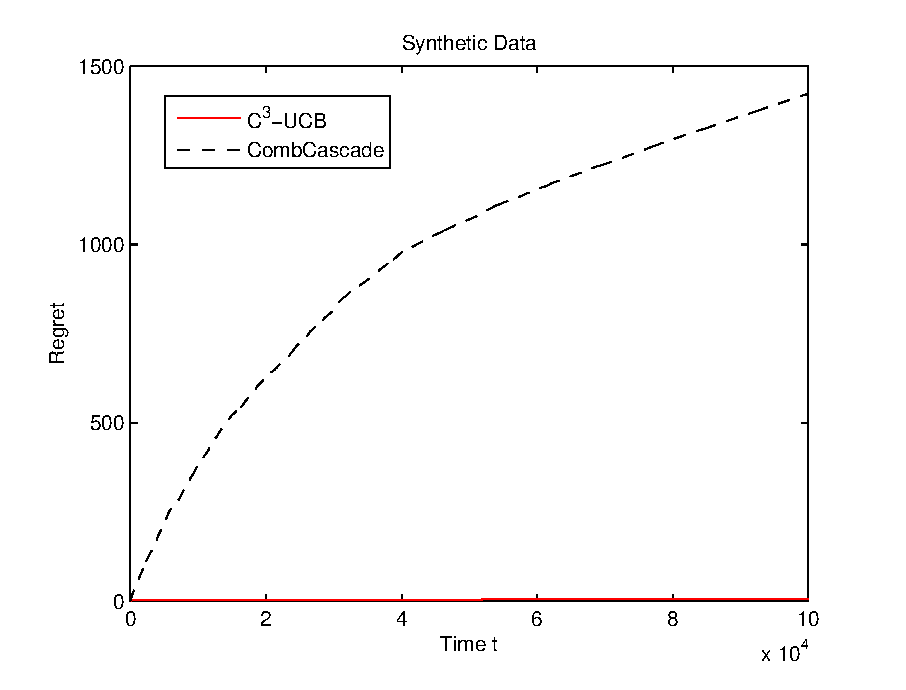
\includegraphics[height = 3 cm, width = 4 cm]{synD-T5-L100-K4-1.eps}}
	\subfigure[Disjunctive, $\gamma=0.9$]{
		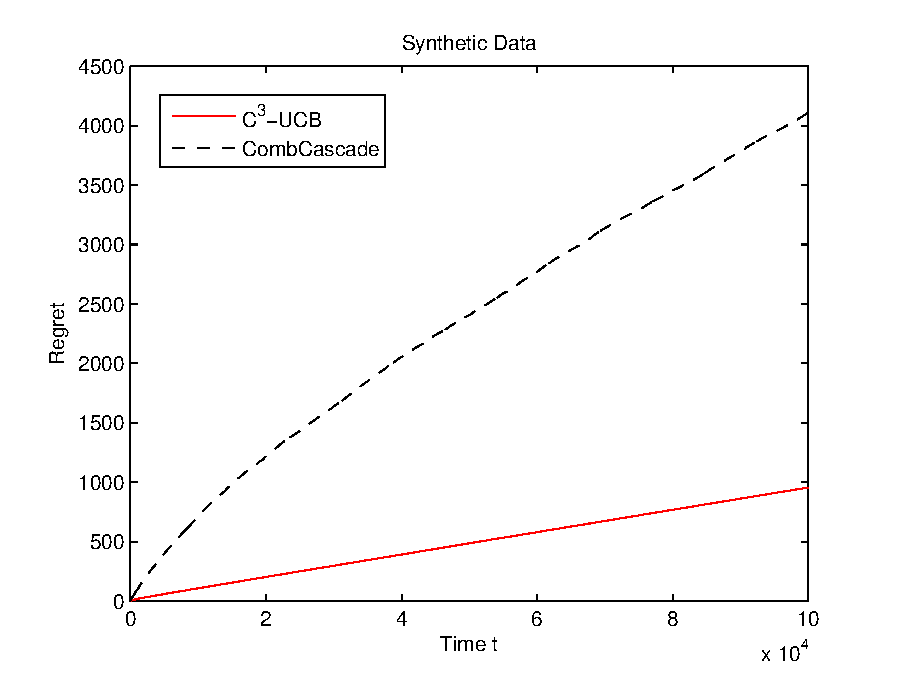
\includegraphics[height = 3 cm, width = 4 cm]{synD-T5-L100-K4-9.eps}}
	\subfigure[Conjunctive, $\gamma=1$ ]{
		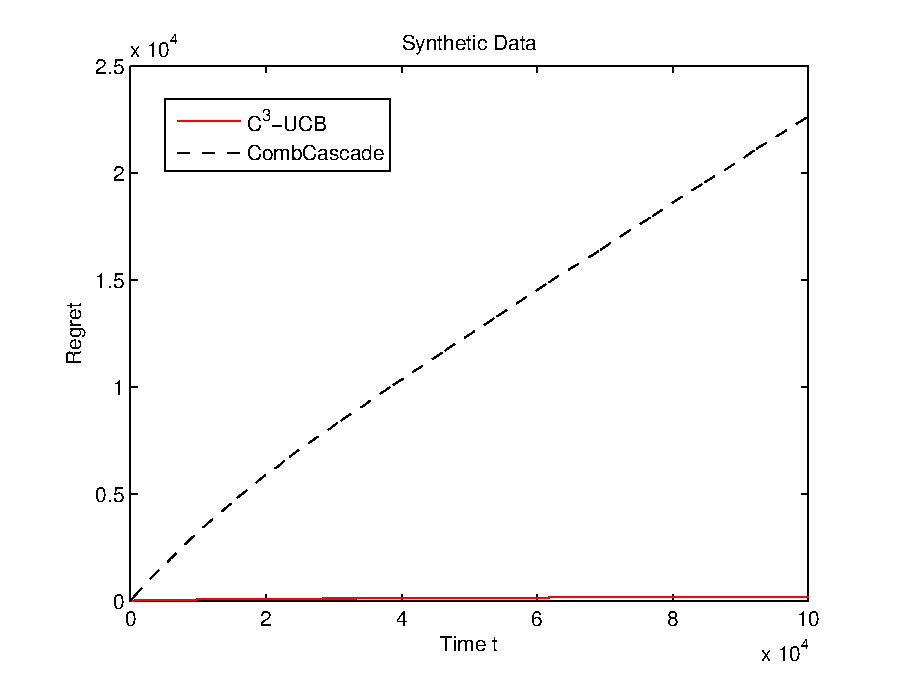
\includegraphics[height = 3 cm, width = 4 cm]{synC-T5-L100-K4-1.eps}}
	\subfigure[Conjunctive, $\gamma=0.9$ ]{
		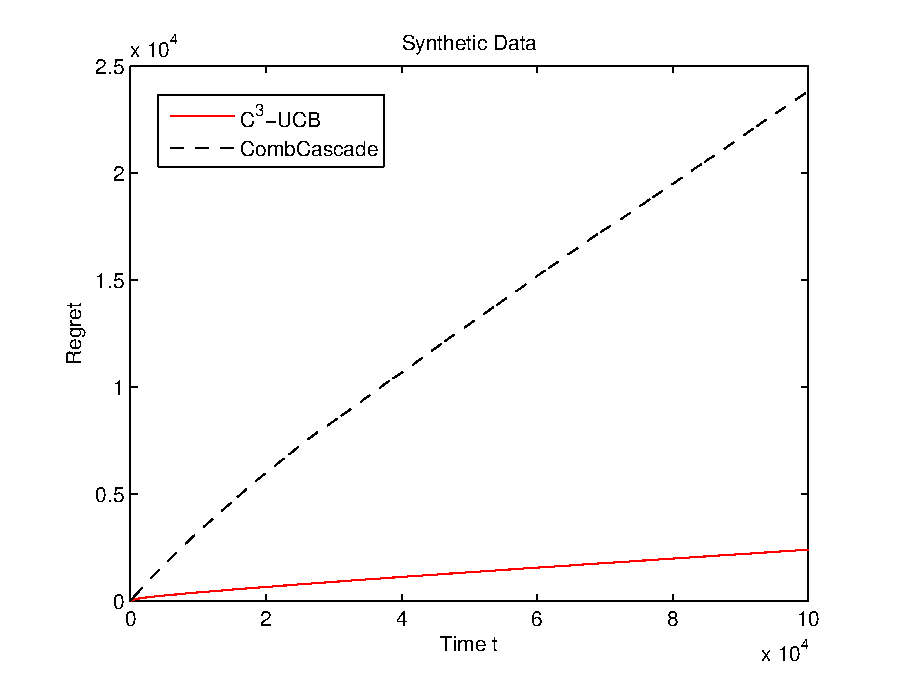
\includegraphics[height = 3 cm, width = 4 cm]{synC-T5-L100-K4-9.eps}}
	\caption{Synthetic Data Set, L=100, K=4, d=10}
	\label{fig:synthetic} % 用于交叉引用
\end{figure*}

\begin{figure}
	\centering
	\subfigure[$\gamma = 1$]{
		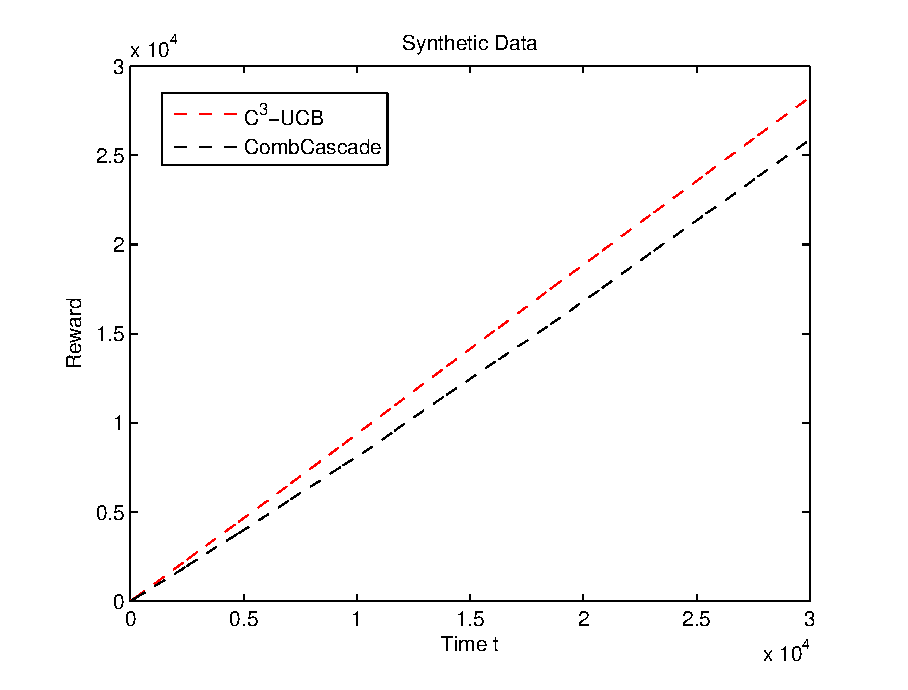
\includegraphics[height = 3cm, width = 3.95 cm]{movieT30000-L200-K4-1.eps}}
	\subfigure[$\gamma = 0.9$]{
		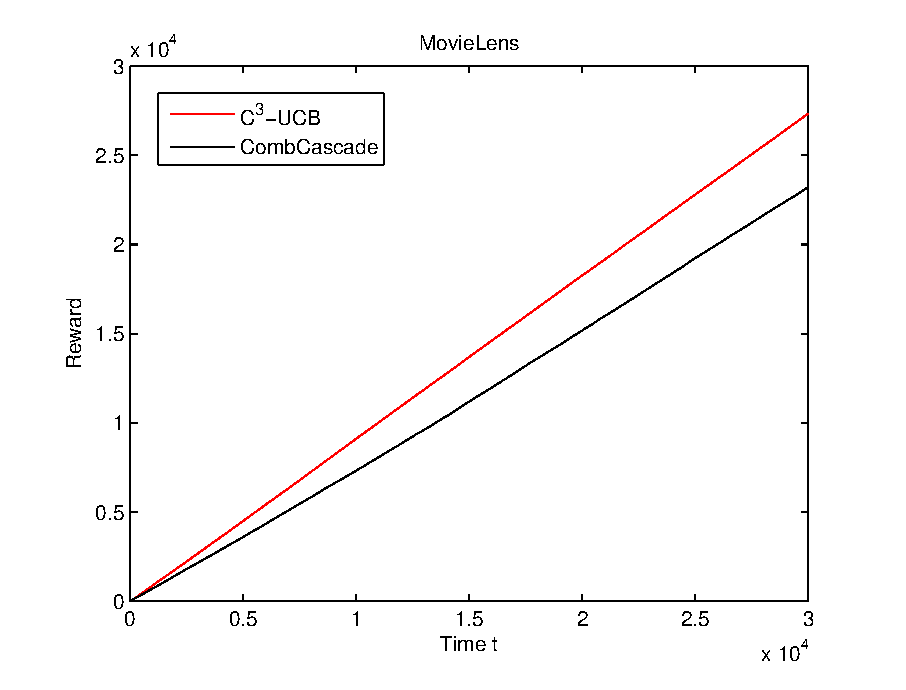
\includegraphics[height = 3cm, width = 3.95 cm]{movieT30000-L200-K4-9.eps}}
	\caption{MovieLens}
	\label{fig:movielens} % 用于交叉引用
\end{figure}

\begin{figure*}
	\centering
	\subfigure[Network 1221]{
		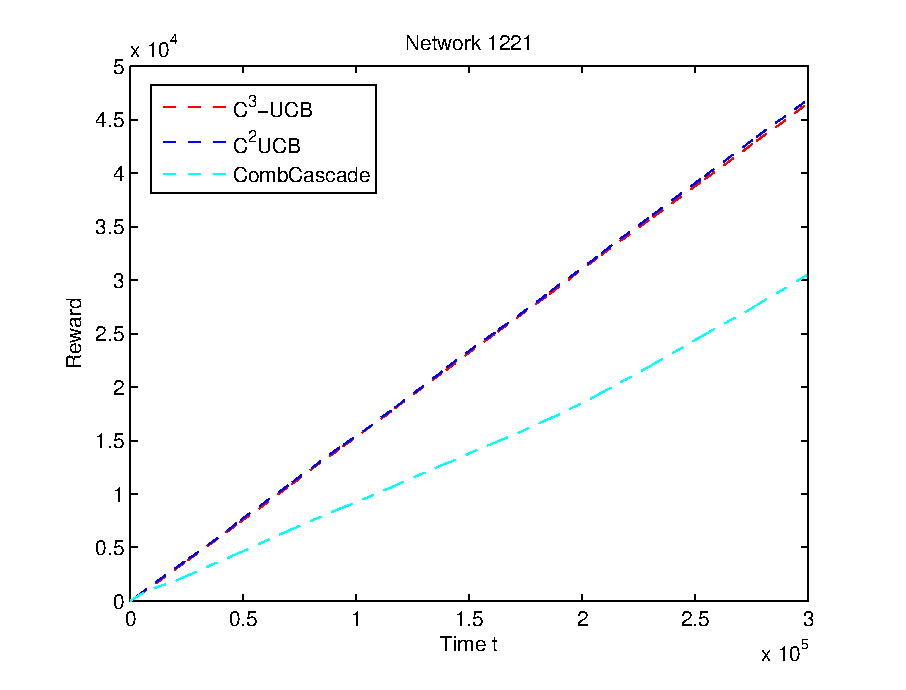
\includegraphics[height = 3 cm, width = 5 cm]{network1-1.eps}}
	\subfigure[Network 1755]{
		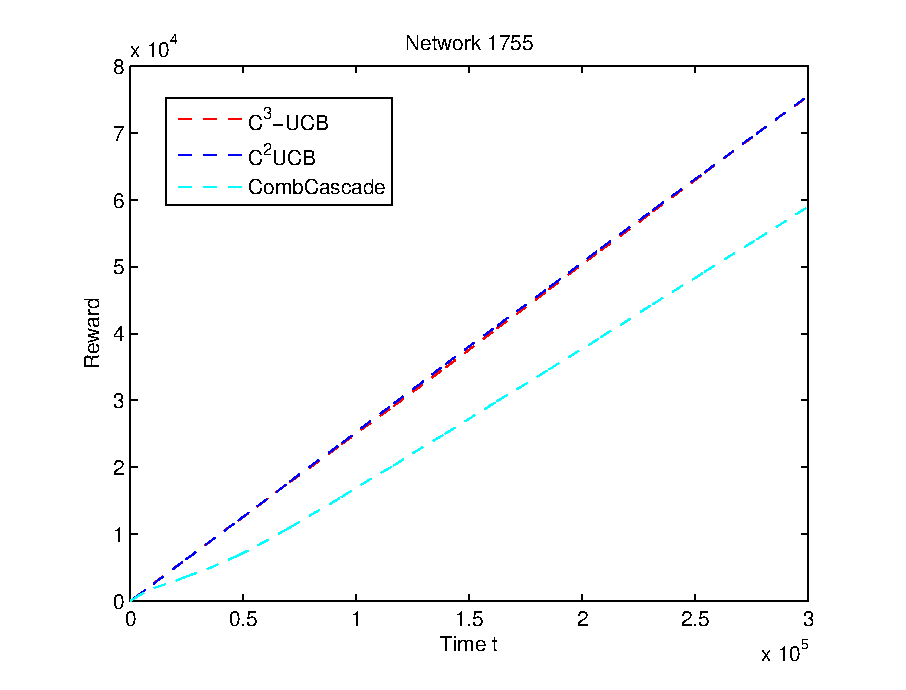
\includegraphics[height = 3 cm, width = 5 cm]{network3-1.eps}}
	\subfigure[Network 3257 ]{
		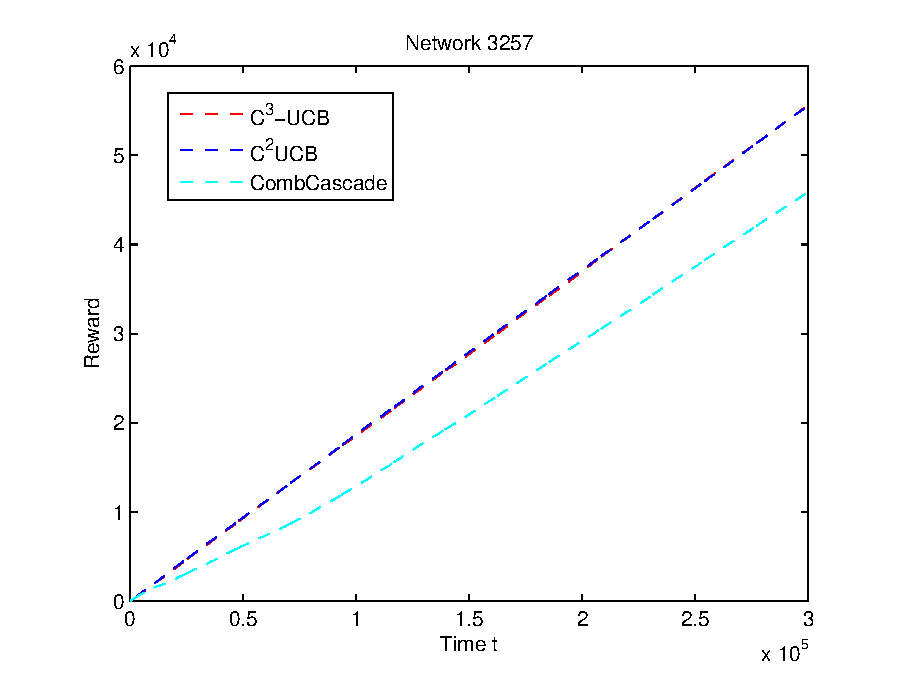
\includegraphics[height = 3 cm, width = 5 cm]{network4-1.eps}}
	\caption{Network with latency}
	\label{fig:network} % 用于交叉引用
\end{figure*}

\section{Experiments}

We evaluate $C^3$-UCB in three experiments. In the following experiments, we let the position discounts $\gamma_k, k\leq K$ have the form of $\gamma^{k-1}$ for some $\gamma$. 

\subsection{Synthetic}
\label{sec:ExpSyn}

In the first experiment, we compare $C^3$-UCB to CombCascade on synthetic problems. This problem is a contextual cascading bandit with $L=100$ items and $K=4$, where at each time $t$ the agent recommends $K$ items to the user. At first, we randomly choose $\theta \in \RR^{d-1}$ with $\|\theta \|_2 = 1$ and let $\theta_* = (\frac{\theta}{2}, \frac{1}{2})$. Then at each time $t$, we randomly assign $x'_{t,a} \in \RR^{d-1}$ with $\|x_{t,a}\| = 1$ to arm $a$ and use $x_{t,a} = (x'_{t,a}, 1)$ to be the context information for arm $a$. This processing will guarantee the inner product $\theta_*^{\top}x_{t,a} = \frac{\theta^{\top}x + 1}{2} \in [0,1]$. Next we generate the weight for arm $a$ at time $t$ by a random sample from Bernoulli distribution with mean $\theta_*^{\top}x_{t,a}$.

We experiment on four settings. Under each setting, the learning agent chooses a set of $K$ items out of $L$ ground items. The first two are of the disjunctive objective where the learning agent observes from the first one of the chosen $K$ items until first one with weight $1$; the last two are of conjunctive objective where the learning agent observes from the first item until the first one with weight $0$. Notice that with $\gamma \leq 1$, the oracle to select a feasible action is to select the set of $K$ items with highest UCBs; $\gamma < 1$ will force the items in the optimal action list in the decreasing order of their UCBs and we also use this order when $\gamma = 1$. The results are shown in Fig.~\ref{fig:synthetic} and our algorithm outperforms {\it CombCascade} algorithm because they do not make use of the context information.


\subsection{MovieLens}

In this experiment, we evaluate $C^3$-UCB on a problem of contextual recommendations. We experiment on {\it MovieLens} dataset\cite{lam2013movie} of 2015.

The Learning problem is formulated as follows. There is a big sparse matrix $A \in \{0,1\}^{N_1 \times N_2}$ where $A(i,j) = 1$ denotes user $i$ has watched movie $j$. We split $A$ to be $H + F$ by putting entry-$1$ in $A$ to $H$ and $F$ with probability $\sim \mathrm{Ber}(p)$ for some fixed $p$. We can regard $H$ as known information about history 'what users have watched' and regard $F$ as future criterion. We use $H$ to derive feature vectors of both users and movies by SVD decomposition, $H = USM^{\top}$ where $U = (u_1; ...;u_{N_1})$ and $M = (m_1;...;m_{N_2})$. At every time $t$, use $x_{t,i} = u_{i}m_j^{\top}$ as the context information of base arm $i$ and randomly choose a user $I_t$. And use $w_t(m) = F(I_t,m)$ as the weight of movie $m$ at time $t$.

This problem is required to recommend fixed number of movies. Notice that it might have problem if we use $(u_{I_t}, m_j)$ as context information. Denote $\theta$ by $(\theta_u, \theta_m)$. So the expected mean of a base arm is of the form $\theta_u^{\top} u_{I_t} + \theta_m^{\top} m_j$ but the first term $\theta_u^{\top} u_{I_t}$ is fixed at time $t$ no matter what $\theta_u$ is. Therefore, to find the best super arm, it is equivalent to rank the scores $\theta_m^{\top} m_j$ for each movie $j$. So to make use of the user's context information, we need some quadratic terms of user's information $u_i$ and movie's information $m_j$. That's why we use the convolution $u_{i}m_j^{\top}$ to denote the context of movie $j$ at time $t$.

We experiment with different position discount and compare our algorithm with {\it CombCascade}. We show the results in Fig.~\ref{fig:movielens}. Our algorithms outperforms theirs, which demonstrate the advantage of introducing context information in real applications.

\subsection{Network Routing}

In the last experiment, we evaluate $C^3$-UCB on a problem of network routing. We experiment on six networks from the {\it RocketFuel} dataset\cite{spring2004measuring}.

The ground set $E$ is the set of links in the network and the feasible action set $\cS$ is the set of all paths in the network. Before learning, the environment randomly chooses a $d$-dimensional vector $\theta_* \in [0,1]^d$ and at each time $t$, any link $e$ is assigned with a random $d$-dimensional context vector $x_{t,e}$. Notice here both $\theta$ and $x$ have been processed like section \ref{sec:ExpSyn} so that $\theta_*^{\top}x \in [0,1]$. The weight for each edge $e$ is a Bernoulli random variable with mean $\theta_*^{\top}x$.

At each time $t$, A pair of source and terminal nodes $(v_s, v_t)$ are chosen randomly. The learning agent recommends a feasible path $A = (a_1,...,a_{|A|})$ between $v_s$ and $v_t$ to maximize the expected reward in the conjunctive objective.

We experiment with different position discounts and on different networks. The results are shown in Fig.~\ref{fig:network}. Our algorithm ourperforms {\it CombCascade} algorithm.

% we randomly generate a pair of starting and ending nodes, and the learning agent chooses a routing path between the two nodes to maximize the expected reward with position discount.

%  and the corresponding latency follows exponential distribution with mean $1-\theta^{\top}x$, which has been scaled into $[0,1]$. We call the latency is {\it high} if it is larger than a threshold $\tau$. 
% $$
% \prod_{k=1}^{|A|} (1- \exp(-\frac{\tau}{1-\theta^{\top}x_{t,a_k}})).
% $$
% Notice that the expression is not of the form $\prod_{k=1}^{|A|}\theta_*^{\top}x_{t,a_k}$ in our model. However, our algorithm could also apply to it.

% the environment randomly choose 

\section{Conclusions}

In this paper, we propose contextual combinatorial cascading bandits, a class of contextual combinatorial bandits with partial observations. 


% In the unusual situation where you want a paper to appear in the
% references without citing it in the main text, use \nocite
%\nocite{langley00}
	
\bibliography{cascade_reference}
\bibliographystyle{icml2016}

\appendix

\section{Proof of Theorem~\ref{thm:main}}

The following lemma provides the important result on the regret at each time $t$ in terms of feature vectors of base arms at the time.

\begin{lemma} %lem:DeltaEstimate
	\label{lem:DeltaEstimate}
	For any time $t$ and $A = (a_1, \ldots, a_{\abs{A}})$, if $f$ satisfies the two assumptions, the properties of monotonicity and Lipschitz continuity, 
	%and $f(A_t^*, \bU_t) \leq f(A, \bU_t)$, 
	then we have
	$$
		R(t, \bA_t) \leq B \sum_{k=1}^{\abs{\bA_t}} \gamma_k \bbeta_{t-1}(\delta)\norm{x_{t, \ba_k}}_{\bV_{t-1}^{-1}}.
	$$
\end{lemma}
\begin{proof}
	By Lemma \ref{lem:estimateU}, $w_t \leq \bU_t$. Then
	\begin{align*}
		f(\bA_t, \bU_t) \geq \alpha f(\bA_t^{\bU_t}, \bU_t) \geq \alpha f(A_t^*, \bU_t) \geq \alpha f(A_t^*, w_t),
	\end{align*}
	where $f(\bA_t^{\bU_t}, \bU_t) = \max_{A \in \cS} f(A, \bU_t)$. The first inequality is because we choose $\bA_t$ by the $\alpha$-approximation oracle with input $\bU_t$; the second inequality is because the maximum of $f(\bA_t^{\bU_t}, \bU_t)$ given $\bU_t$; the third inequality is by the monotonicity of $f$ and the property $\bU_t \geq w_t$. Then
	\begin{align*}
		R(t, \bA_t) = &\alpha f(A_t^*, w_t) - f(\bA_t, w_t) \\
		\leq &f(\bA_t, \bU_t) - f(\bA_t, w_t).
	\end{align*}
	By Lipschitz continuity of $f$ and the definition of $\bU_t$ in Eq.\eqref{eq:defU},
	$$
	f(\bA_t, \bU_t) \leq f(\bA_t, \theta_{\ast}^{\top}x_t) + B \sum_{k=1}^{\abs{\bA_t}} \gamma_k \bbeta_{t-1}(\delta)\norm{x_{t, \ba_k^t}}_{\bV_{t-1}^{-1}}.
	$$
	Then we have
	\begin{align*}
		R(t, A) \leq &f(\bA_t, \bU_t) - f(\bA_t, w_t) \\
		\leq &B \sum_{k=1}^{\abs{\bA_t}} \gamma_k \bbeta_{t-1}(\delta)\norm{x_{t, \ba_k^t}}_{\bV_{t-1}^{-1}}.
	\end{align*}
\end{proof}

Notice that the upper bound of $R(t, \bA_t)$ is in terms of all base arms of $\bA_t$. However, it is hard to estimate an upper bound for $\sum_{t=1}^T \sum_{k=1}^{\abs{\bA_t}} \norm{ x_{t, \ba_k^t} }_{ \bV_{t-1}^{-1} }$ because $\bV_t$ only contains information of observed base arms. Thus we need the following lemma.

\begin{lemma} %lem:DeltaEsimateWithP*
	\label{lem:DeltaEsimateWithP*}
	Suppose the equation (\ref{eq:estimateTheta}) holds for time $t-1$. Then
	$$
	\EE_t[R(t, \bA_t)] \leq \frac{B}{p^*} \EE_t \left[ \bbeta_{t-1}(\delta) \sum_{k=1}^{\bO_t}\norm{\gamma_k x_{t,\ba_k^t}}_{\bV_{t-1}^{-1}} \right].
	$$
\end{lemma}
\begin{proof}
	\begin{align}
		&\EE[R(t, \bA_t)|\cH_t]  \nonumber \\
		=& \EE \left[ \left. R(t, \bA_t) \EE \left[ \left. \frac{1}{p_{t, \bA_t}} \bOne\{\bO_t = \abs{\bA_t}\} \right| \bA_t \right]  \right| \cH_t \right] \label{eq:addOt}\\
		=& \EE \left[ \left. R(t, \bA_t) \frac{1}{p_{t, \bA_t}} \bOne\{\bO_t = \abs{\bA_t}\}  \right| \cH_t \right] \label{eq:removeE}\\
		\leq &\frac{1}{p^{\ast}} \EE \left[ \left. R(t, \bA_t) \bOne\{\bO_t = \abs{\bA_t}\}  \right| \cH_t \right] \label{eq:relaxpstar}\\
		\leq &\frac{B}{p^{\ast}} \EE \left[ \left. \sum_{k=1}^{\abs{\bA_t}} \gamma_k \bbeta_{t-1}(\delta)\norm{x_{t,a_k}}_{\bV_{t-1}^{-1}} \bOne\{\bO_t = \abs{\bA_t}\}  \right| \cH_t \right] \label{eq:useradiusbound}\\
		\leq &\frac{B}{p^{\ast}} \EE \left[ \left. \sum_{k=1}^{\bO_t} \gamma_k \bbeta_{t-1}(\delta)\norm{x_{t,a_k}}_{\bV_{t-1}^{-1}} \right| \cH_t \right]. \label{eq:relaxindicator}
	\end{align}
	Equality \eqref{eq:addOt} is because when $\bA_t$ is fixed, $p_{t, \bA_t}$ is the probability of $\bO_t = \abs{\bA_t}$, and thus the inner expectation is $1$. Equality \eqref{eq:removeE} is because when the history $\cH_t$ is fixed, $\bA_t$ is fixed by the deterministic algorithm C$^3$-UCB, and thus there is no need to write the conditional expectation. Inequality~\eqref{eq:relaxpstar} is because $p_{t,\bA_t} \geq p^*$ by definition. Inequality~\eqref{eq:useradiusbound} is by Lemma \ref{lem:DeltaEstimate} and the fact $f(A_t^*, \bU_t) \leq f(\bA_t, \bU_t)$, which is true because algorithm C$^3$-UCB selects action $\bA_t$ as the best action with respect to $\bU_t$. Inequality~\eqref{eq:relaxindicator} is by simply arguing on the two cases for the indicator function $\bOne\{\bO_t = \abs{\bA_t}\}$.
\end{proof}


% \begin{lemma} %lem:DeltaEstimate
%   \label{lem:DeltaEstimate}
%   For any time $t$ and $A = (a_1, \ldots, a_{\abs{A}})$, if $f(A_t^*, \bU_t) \leq f(A, \bU_t)$, then we have
%   $$
%     R(t,A) \leq \sum_{k=1}^{\abs{A}} \gamma_k \bbeta_{t-1}(\delta)\norm{x_{t,a_k}}_{\bV_{t-1}^{-1}};
%   $$
%   if $f_{\wedge}(A_t^*, \bU_t) \leq f_{\wedge}(A, \bU_t)$, then we have
%   $$
%     R_{\wedge}(t, A) \leq \sum_{k=1}^{\abs{A}} \gamma_k \bbeta_{t-1}(\delta)\norm{x_{t,a_k}}_{\bV_{t-1}^{-1}}.
%   $$
% \end{lemma}
% \begin{proof}
%   By Lemma \ref{lem:estimateU}, $\theta_{\ast}^{\top}x_t \leq \bU_t$. Then by Lemma \ref{lem:increasing},
%   $$
%     f_t^{\ast} = f(A_t^{\ast}, \theta_{\ast}^{\top}x_t) \leq f(A_t^{\ast}, \bU_t).
%   $$
%   By Lemma \ref{lem:estimateTech} and the definition of $\bU_t$ in Eq.\eqref{eq:defU},
%   $$
%     f(A, \bU_t) \leq f(A, \theta_{\ast}^{\top}x_t) + \sum_{k=1}^{\abs{A}} \gamma_k \bbeta_{t-1}(\delta)\norm{x_{t, a_k^t}}_{\bV_{t-1}^{-1}}.
%   $$
%   By our condition that $f(A_t^{\ast}, \bU_t) \leq f(A, \bU_t)$, we have 
%   $$
%     f_t^{\ast} \leq f(A, \theta_{\ast}^{\top}x_t) + \sum_{k=1}^{\abs{A}} \gamma_k \bbeta_{t-1}(\delta)\norm{x_{t, a_k^t}}_{\bV_{t-1}^{-1}}.
%   $$
%   Therefore,
%   $$
%     R(t, A) = f_t^{\ast} - f(A, \theta_{\ast}^{\top}x_t) \leq \sum_{k=1}^{\abs{A}} \gamma_k \bbeta_{t-1}(\delta)\norm{x_{t, a_k^t}}_{\bV_{t-1}^{-1}}.
%   $$
%   The result for the conjunctive case can be deduced in a similar way.
% \end{proof}

% Notice that if we substitute $A$ by $\bA_t$ in Lemma \ref{lem:DeltaEstimate}, then the upper bound of $R(t, \bA_t)$ is in terms of all base arms of $\bA_t$. 
% However, it is hard to estimate an upper bound for $\sum_{t=1}^T \sum_{k=1}^{\abs{\bA_t}} \norm{ x_{t, \ba_k^t} }_{ \bV_{t-1}^{-1} }$ because $\bV_t$ only contains observed base arms. Thus we need the following lemma.

% \begin{lemma} %lem:DeltaEsimateWithP*
%   \label{lem:DeltaEsimateWithP*}
%   Let $1 \geq \gamma_1 \geq \cdots \geq \gamma_K \geq 0$ and $\gamma_k' = 1 - \gamma_k$.
%   Suppose the equation (\ref{eq:estimateTheta}) holds for time $t-1$. Then
%   $$
%     \EE_t[R(t, \bA_t)] \leq \frac{1}{p^*} \EE_t \left[ \bbeta_{t-1}(\delta) \sum_{k=1}^{\bO_t}\norm{\gamma_k x_{t,\ba_k^t}}_{\bV_{t-1}^{-1}} \right].
%   $$
%   If we have
%   $$
%     \gamma_K' \le \frac{1}{4} f_{\wedge}^{\ast} = \frac{1}{4} \min_{1 \leq t \leq T} f_{\wedge, t}^{\ast},
%   $$
%   then
%   $$
%     \EE_t [R_{\wedge}(t, \bA_t) ] \leq \frac{8}{f_{\wedge}^{\ast}} \EE_t \left[ \bbeta_{t-1}(\delta)\sum_{k=1}^{\bO_t}\norm{\gamma_k x_{t,\ba_k^t}}_{\bV_{t-1}^{-1}} \right].
%   $$
% \end{lemma}
% \begin{proof}
%   For the disjunctive case,  
%   \begin{align}
%     &\EE[R(t, \bA_t)|\cH_t]  \nonumber \\
%     =& \EE \left[ \left. R(t, \bA_t) \EE \left[ \left. \frac{1}{p_{t, \bA_t}} \bOne\{\bO_t\geq\abs{\bA_t}\} \right| \bA_t \right]  \right| \cH_t \right] \label{eq:addOt}\\
%     =& \EE \left[ \left. R(t, \bA_t) \frac{1}{p_{t, \bA_t}} \bOne\{\bO_t\geq\abs{\bA_t}\}  \right| \cH_t \right] \label{eq:removeE}\\
%     \leq &\frac{1}{p^{\ast}} \EE \left[ \left. R(t, \bA_t) \bOne\{\bO_t\geq\abs{\bA_t}\}  \right| \cH_t \right] \label{eq:relaxpstar}\\
%     \leq &\frac{1}{p^{\ast}} \EE \left[ \left. \sum_{k=1}^{\abs{\bA_t}} \gamma_k \bbeta_{t-1}(\delta)\norm{x_{t,a_k}}_{\bV_{t-1}^{-1}} \bOne\{\bO_t\geq\abs{\bA_t}\}  \right| \cH_t \right] \label{eq:useradiusbound}\\
%     \leq &\frac{1}{p^{\ast}} \EE \left[ \left. \sum_{k=1}^{\bO_t} \gamma_k \bbeta_{t-1}(\delta)\norm{x_{t,a_k}}_{\bV_{t-1}^{-1}} \right| \cH_t \right]. \label{eq:relaxindicator}
%   \end{align}
%   Equality \eqref{eq:addOt} is because when $\bA_t$ is fixed, $p_{t, \bA_t}$ is the probability of $\bO_t\geq\abs{\bA_t}$, and thus the inner expectation is $1$. 
%   Equality \eqref{eq:removeE} is because when the history $\cH_t$ is fixed, $\bA_t$ is fixed by the deterministic algorithm C$^3$-UCB, and thus there is no need to write the conditional expectation. 
%   Inequality~\eqref{eq:relaxpstar} is because $p_{t,\bA_t} \geq p^*$ by definition. 
%   Inequality~\eqref{eq:useradiusbound} is by Lemma \ref{lem:DeltaEstimate} and the fact $f(A_t^*, \bU_t) \leq f(\bA_t, \bU_t)$, which is true because algorithm C$^3$-UCB selects action $\bA_t$ as the best action with respect to $\bU_t$. 
%   Inequality~\eqref{eq:relaxindicator} is by simply arguing on the two cases for the indicator function $\bOne\{\bO_t\geq\abs{\bA_t}\}$.
  
%   For the conjunctive case, by Lemma~\ref{lem:prefixexists} there exists a prefix $\bB_t$ of $\bA_t$ such that $p_{\wedge, t, \bB_t} \geq \frac{1}{2}f_{\wedge, t}^* - \gamma'_{|\bB_t|}$ and $R_{\wedge}(t, \bB_t) \geq \frac{1}{2} R_{\wedge}(t, \bA_t)$. 
%   By the assumption that $\gamma'_{|\bB_t|}\le \gamma'_K \le \frac{1}{4} f^*_{\wedge} \le \frac{1}{4} f^*_{\wedge,t}  $, we have $p_{\wedge, t, \bB_t} \geq \frac{1}{4}f_{\wedge, t}^*$. 
%   Then, similar to the derivation from Eq.\eqref{eq:addOt} to Eq.\eqref{eq:relaxpstar}, we have
%   \begin{align}
%     &\EE_t[R_{\wedge}(t, \bA_t)] \leq 2 \EE[R_{\wedge}(t, \bB_t) \left. \right| \cH_t] \nonumber \\
%     =& 2 \EE \left[ \left. R_{\wedge}(t, \bB_t) \EE \left[ \left. \frac{1}{p_{\wedge, t, \bB_t}} \bOne\{\bO_t\geq\abs{\bB_t}\} \right| \bB_t \right]  \right| \cH_t \right] \nonumber \\
%     =& 2\EE \left[ \left. R_{\wedge}(t, \bB_t) \frac{1}{p_{\wedge, t, \bB_t}} \bOne\{\bO_t\geq\abs{\bB_t}\}  \right| \cH_t \right] \nonumber \\
%     \leq &\frac{8}{f_{\wedge, t}^{\ast}} \EE \left[ \left. R_{\wedge}(t, \bB_t) \bOne\{\bO_t\geq\abs{\bB_t}\}  \right| \cH_t \right]. \label{eq:btOneotbt}
%   \end{align}
%   Next, we have
%   \begin{equation} \label{eq:andstarbt}
%     f_{\wedge}(A_t^*, \theta_*^{\top}x_t) \leq f_{\wedge}(A_t^*,\bU_t) \leq f_{\wedge}(\bA_t,\bU_t) \leq f_{\wedge}(\bB_t,\bU_t),
%   \end{equation}
%   where the first inequality is by Lemmas \ref{lem:estimateU} and \ref{lem:increasing}, the second inequality is by the C$^3$-UCB algorithm, in which the best action $\bA_t$ is selected with respect to $\bU_t$, and the last inequality is by Lemma~\ref{lem:prefixRelation}~(2).
  
%   Then by Lemma \ref{lem:estimateTech},
%   \begin{equation} \label{eq:btuttrue}
%     f_{\wedge}(\bB_t,\bU_t) \leq f_{\wedge}(\bB_t, \theta_*^{\top}x_t) + \sum_{k=1}^{\abs{\bB_t}}\gamma_k\bbeta_{t-1}(\delta)\norm{x_{t,\ba_k^t}}_{\bV_{t-1}^{-1}}.
%   \end{equation}
%   Therefore, combining Eq.\eqref{eq:andstarbt} and \eqref{eq:btuttrue}, we have
%   \begin{align}
%     R_{\wedge}(t, \bB_t) & = f_{\wedge, t}^{\ast} - f_{\wedge}(\bB_t, \theta_{\ast}^{\top}x_t) \nonumber \\
%     & \leq \sum_{k=1}^{\abs{\bB_t}}\bbeta_{t-1}(\delta)\norm{\gamma_k x_{t,\ba_k^t}}_{\bV_{t-1}^{-1}}. \label{eq:sumbetax}
%   \end{align}
%   Finally from Inequalities~\eqref{eq:btOneotbt} and \eqref{eq:sumbetax}, we can derive the result
%   \begin{align*}
%     &\EE_t[R_{\wedge}(t, \bA_t)] \\
%     \leq& \frac{8}{f_{\wedge, t}^*} \EE \left[\bOne\{ \bO_t \geq \abs{\bB_t} \}\sum_{k=1}^{\abs{\bB_t}}\bbeta_{t-1}(\delta)\norm{\gamma_k x_{t,\ba_k^t}}_{\bV_{t-1}^{-1}} \right]\\
%     \leq& \frac{8}{f_{\wedge}^*} \EE \left[ \sum_{k=1}^{ \bO_t } \bbeta_{t-1}(\delta) \norm{\gamma_k x_{t,\ba_k^t}}_{\bV_{t-1}^{-1}} \right].
%   \end{align*}
% \end{proof}

From the above lemma, we can bound the regret at time $t$ in terms of the observed base arms, for which we further bound in Lemma~\ref{lem:SumXiEstimateInDet}.
But before that, we need the following technical lemma.

\begin{lemma} %lem:detTech
  \label{lem:detTech}
  Let $x_i \in \RR^{d \times 1}, 1 \leq i \leq n$. Then we have
  $$
    \det\left(I + \sum_{i=1}^n x_i x_i^{\top}\right) \geq 1 + \sum_{i=1}^n \norm{x_i}_2^2.
  $$
\end{lemma}
\begin{proof}
  Denote the eigenvalues of $I + \sum_{i=1}^n x_i x_i^{\top}$ by $1+\alpha_1,...,1+\alpha_d$ with $\alpha_j \geq 0$, $1\leq j\leq d$. Then
  \begin{align*}
    &\det(I + \sum_{i=1}^n x_i x_i^{\top})= \prod_{j=1}^d (1 + \alpha_j)\\
    &\geq 1 +\sum_{j=1}^d \alpha_j =1-d + \sum_{i=1}^d (1+\alpha_i) \\
    &=1-d + \trace(I + \sum_{i=1}^n x_i x_i^{\top})= 1-d + d + \sum_{i=1}^n \norm{x_i}_2^2\\
    &=1 + \sum_{i=1}^n \norm{x_i}_2^2.
  \end{align*}
\end{proof}


\begin{lemma} % lem:SumXiEstimateInDet
  \label{lem:SumXiEstimateInDet}
  \CLemmaSumXiEstimateInDet
\end{lemma}
\begin{proof}
	\begin{align}
	&\det(\bV_t) = \det\left(\bV_{t-1} + \sum_{k=1}^{\bO_t} (\gamma_k x_{t,\ba_k^{t}})(\gamma_k x_{t, \ba_k^{t}}^{\top}) \right) \nonumber \\
	&=\det(\bV_{t-1}) \notag \\
	&~~~\cdot \det \left(I + \sum_{k=1}^{\bO_t} \gamma_k \bV_{t-1}^{-1/2}x_{t,\ba_{k}^{t}} (\gamma_k \bV_{t-1}^{-1/2}x_{t,\ba_{k}^{t}})^{\top} \right) \label{eq:Vfactor}\\
	&\geq \det(\bV_{t-1}) \left(1 + \sum_{k=1}^{\bO_t} \norm{\gamma_k x_{t,\ba_k^t}}_{\bV_{t-1}^{-1}}^2 \right) \label{eq:detGeq} \\
	&\geq \det(\lambda I)\prod_{s=1}^{t} \left(1 + \sum_{k=1}^{\bO_s} \norm{\gamma_k x_{s,\ba_k^s}}_{\bV_{s-1}^{-1}}^2 \right), \label{eq:repeatV}
	\end{align}
	where Equality~\eqref{eq:Vfactor} is by the fact that $V+U = V^{1/2} (I + V^{-1/2} U V^{-1/2}) V^{1/2}$ for a symmetric positive definite matrix $V$, Inequality \eqref{eq:detGeq} is due to Lemma \ref{lem:detTech}, and Inequality~\eqref{eq:repeatV} is by repeatedly applying Inequality \eqref{eq:detGeq}.
	
	Because
	$$
	\norm{\gamma_k x_{s,\ba_k^s}}_{\bV_{s-1}^{-1}}^2 \leq \norm{\gamma_k x_{s,\ba_k^s}}_2^2/\lambda_{\min}(\bV_{s-1}) \leq \gamma_k^2 /\lambda,
	$$
	where $\lambda_{\min}(\bV_{s-1})$ is the minimum eigenvalue of $\bV_{s-1}$,  we have 
	$$
	\sum_{k=1}^{\bO_s} \norm{\gamma_k x_{s,\ba_k^s}}_{\bV_{s-1}^{-1}}^2 \leq \frac{1}{\lambda} \sum_{k=1}^{K} \gamma_k^2 = C_\gamma /\lambda \leq 1
	$$
	Using the fact that $ 2\ln(1+u) \geq u$ for any $u \in [0,1]$, we get
	\begin{align*}
	&\sum_{s=1}^t \sum_{k=1}^{\bO_s}\norm{\gamma_k x_{s,\ba_{k}^s}}_{\bV_{s-1}^{-1}}^2 \\
	&\leq 2\sum_{s=1}^t\ln \left(1 + \sum_{k=1}^{\bO_s} \norm{\gamma_k x_{s,\ba_k^s}}_{\bV_{s-1}^{-1}}^2 \right)\\
	& = 2 \ln \prod_{s=1}^{t} \left(1 + \sum_{k=1}^{\bO_s} \norm{\gamma_k x_{s,\ba_k^s}}_{\bV_{s-1}^{-1}}^2 \right) \\
	&\le 2 \ln \left(\frac{\det(\bV_t)}{\det(\lambda I)} \right),
	\end{align*}
	where the last inequality is from Inequality~\eqref{eq:repeatV}.
\end{proof}

Finally the last lemma bounds $\det(\bV_t)$.

\begin{lemma} % det(V_t)
	\label{lem:detVt}
	\CLemmaDetVt
\end{lemma}
\begin{proof}
	To prove $\det(\bV_t)$ is increasing with respect to $t$, it is enough to prove that
	$$
	\det(V + xx^{\top}) \geq \det(V),
	$$
	for any symmetric positive definite matrix $V \in \RR^{d \times d}$ and column vector $x \in \RR^{d\times 1}$. In fact,
	\begin{align*}
	&\det(V + xx^{\top}) \\
	=& \det(V) \det(I + V^{-1/2}x x^{\top} V^{-1/2})\\
	=& \det(V) \det(1 + \norm{V^{-1/2}x}^2)\\
	\geq &\det(V).
	\end{align*}
	The second equality above is due to Sylvester's determinant theorem, which states that $\det(I + AB) = \det(I +BA)$.
	
	Let the eigenvalues of $\bV_t$ be $\lambda_1, \ldots, \lambda_d > 0$. Then
	\begin{align*}
	&\det(\bV_t) = \lambda_1 \cdot \cdots \cdot \lambda_d \\
	\leq & \left( \frac{\lambda_1 + \ldots + \lambda_d}{d} \right)^d = (\trace(\bV_t)/d)^d.
	\end{align*}
	Also,
	\begin{align*}
	&\trace(\bV_t)\\
	& = \trace(\lambda I) + \sum_{s=1}^t \sum_{k=1}^{\bO_s} \gamma_k^2 \trace(x_{s,\ba_k^s} x_{s,\ba_k^s}^{\top})\\	
	& = d \lambda + \sum_{s=1}^t \sum_{k=1}^{\bO_s} \gamma_k^2 \norm{x_{s,\ba_k^s}}_2^2\\
	& \leq d \lambda + \sum_{s=1}^t\sum_{k=1}^{K}\gamma_k^2 = d \lambda + t C_\gamma.
	\end{align*}
	Thus we have $\det(\bV_t) \leq (\lambda + C_\gamma t/d)^d.$
\end{proof}

Now we are ready to prove the main theorem.

\begin{proof}[ of Theorem \ref{thm:main}]
	Suppose inequality (\ref{eq:estimateTheta}) holds for all time $t$, which is true with probability $1-\delta$. Then we have
	\begin{align}
	&R(T) = \EE \left[\sum_{t=1}^{n} \EE_{t}[R(t, \bA_t)] \right] \notag\\
	&\leq \EE\left[\sum_{t=1}^{n} \frac{B}{p^*} \EE_t \left[\bbeta_{t-1}(\delta) \sum_{k=1}^{\bO_t}\norm{\gamma_k x_{t,\ba_k^t}}_{\bV_{t-1}^{-1}}\right] \right] \label{eq:pfMdeltaEst}\\
	&\leq \EE\left[\sum_{t=1}^{n} \frac{B}{p^*} \bbeta_{T}(\delta) \EE_t \left[ \sum_{k=1}^{\bO_t}\norm{\gamma_k x_{t,\ba_k^t}}_{\bV_{t-1}^{-1}}\right] \right] \label{eq:pfMbeta}\\
	&\leq \EE \left[\frac{B}{p^*} \bbeta_T(\delta) \sqrt{\left(\sum_{t=1}^{n} \bO_t\right) \left( \sum_{t=1}^{n} \sum_{k=1}^{\bO_t}\norm{\gamma_k x_{t,\ba_k^t}}_{\bV_{t-1}^{-1}}^2 \right)} \right ]  \label{eq:pfMmeanEq}\\
	&\leq \EE\left[\frac{B}{p^*} \left( R \sqrt{ \ln \left( \frac{\det(\bV_n)}{\lambda^d \delta^2} \right)} + \sqrt{\lambda} \right) \right. \notag\\
	& \left. \qquad \qquad \cdot \sqrt{nK \cdot 2\ln \left(\frac{\det(\bV_n)}{\lambda^d} \right)} \right] \label{eq:pfMsumXi}\\
	&\leq \frac{\sqrt{2}B}{p^*} \left(R\sqrt{ d \ln \left( \frac{1 + C_\gamma n/(\lambda d)}{\delta^{2/d}} \right) } + \sqrt{\lambda} \right) \notag\\
	&\qquad \qquad \cdot \sqrt{nKd\ln(1 + C_\gamma n/(\lambda d))}. \label{eq:pfMdetEst}
	\end{align}
	Inequality \eqref{eq:pfMdeltaEst} is by Lemma \ref{lem:DeltaEsimateWithP*}. 
	Inequality \eqref{eq:pfMbeta} is because $\bbeta_{t}(\delta)$ is increasing with respect to $t$, derived by the definition of $\bbeta_t(\delta)$ (Eq.\eqref{eq:definebeta}) and Lemma \ref{lem:detVt}. 
	Inequality \eqref{eq:pfMmeanEq} is by the mean inequality. 
	Inequality \eqref{eq:pfMsumXi} is because of the definition of $\bbeta_t(\delta)$ (Eq.\eqref{eq:definebeta}) and Lemma \ref{lem:SumXiEstimateInDet}. 
	And the last inequality \eqref{eq:pfMdetEst} is because estimate of $\det(\bV_t)$ by Lemma \ref{lem:detVt}.
\end{proof}

\section{Proof of Corollary~\ref{cor:or}}

In this section, we prove the expected reward function
$$
f(A,w) = \sum_{k = 1}^{\abs{A}} \gamma_{k} \prod_{i=1}^{k-1} (1 - w(a_i)) w(a_k),
$$
where $A = (a_1, \ldots, a_{|A|})$, defined in~Eq.\eqref{eq:OrRewardFunc}, satisfies the properties of monotonicity and Lipschitz continuity.

\begin{lemma}[monotonicity]
	\label{lem:orMonotonicity}
	Suppose $1 \geq \gamma_1 \geq \cdots \geq \gamma_K \geq 0$. Then $f(A, w)$ is increasing with respect to $w$; that is, if $0 \leq w \leq w' \leq 1$ as column vectors in $\RR^L$, then for any $A \in \prod^{\leq K}$, it holds that
	$$
	f(A, w) \leq f(A, w').
	$$
\end{lemma}
\begin{proof}
	Without the loss of generality, we prove for the case of $A = (1, \ldots, m)$, where $1 \leq m \leq K$. First, for $1 \leq k \leq m$, we have
	\begin{align*}
		&\gamma_{k} - \sum_{i=k+1}^m \gamma_i \prod_{j = k + 1}^{i - 1} (1 - w_j') w_i'\\
		\geq &~\gamma_k [1 - \sum_{i=k+1}^m \prod_{j=k+1}^{i-1}(1 - w_j') w_i']\\
		\geq &~\gamma_{k} \cdot 0 = 0.
	\end{align*}
	Then it implies that
	\begin{align*}
		&\gamma_k w_k + (1 - w_k)\sum_{i=k+1}^m \gamma_i \prod_{j=k+1}^{i-1}(1 - w_j') w_i'\\
		\leq &\gamma_k w_k' + (1 - w_k')\sum_{i=k+1}^m \gamma_i \prod_{j=k+1}^{i-1}(1 - w_j') w_i'.\\
	\end{align*}
	Therefore, 
	\begin{align*}
		& f(A; w_1, \dots, w_k, w_{k+1}', \dots, w_m')\\
		&=\sum_{i=1}^{k-1} \gamma_i \prod_{j=1}^{i-1}(1 - w_j) w_i + \prod_{j=1}^{k-1}(1 - w_j) \\
		&\qquad \cdot [\gamma_k w_k + (1 - w_k)\sum_{i=k+1}^m \gamma_i \prod_{j=k+1}^{i-1}(1 - w_j') w_i']\\
		&\leq \sum_{i=1}^{k-1} \gamma_i \prod_{j=1}^{i-1}(1 - w_j) w_i + \prod_{j=1}^{k-1}(1 - w_j) \\
		&\qquad \cdot [\gamma_k w_k' + (1 - w_k')\sum_{i=k+1}^m \gamma_i \prod_{j=k+1}^{i-1}(1 - w_j') w_i']\\
		&=f(A; w_1, \ldots, w_{k-1}, w_{k}', \ldots, w_m').
	\end{align*}
\end{proof}

\begin{lemma}[Lipschitz continuity]
	\label{lem:orLip}
	Suppose $0 \leq \gamma_k \leq 1, k \leq K$. Let $w, w'\in [0,1]^{L}$. Then
	$$
	|f(A, w) - f(A, w')| \leq \sum_{k=1}^{|A|} \gamma_k |w(a_k) - w'(a_k)|,
	$$
	where $A = (a_1, \ldots, a_{|A|})$.
\end{lemma}
\begin{proof}
	Without the loss of generality, we prove for the case of $A = (1, \ldots, m)$, where $1 \leq m \leq K$. First, suppose $w \leq w'$ and $w' = w + v$.
	
	We prove this by induction. It holds obviously for $m = 1$. Suppose it holds for $m$. Then
	\begin{align*}
		&f(A^{(m+1)}, w')\\
		=&f(A^{(m)}, w') + \gamma_{m+1}\prod_{k=1}^m(1 - w'_k) w'_{m+1}\\
		\leq &f(A^{(m)}, w') +  \gamma_{m+1} \prod_{k=1}^m(1 - w_k) (w_{m+1} + v_{m+1})\\
		\leq &f(A^{(m)}, w) + \sum_{k=1}^m \gamma_k v_k \\
		&\qquad + \gamma_{m+1} \prod_{k=1}^m(1 - w_k) w_{m+1} + \gamma_{m+1} v_{m+1}\\
		=& f(A^{(m+1)}, w) + \sum_{k=1}^{m+1} \gamma_k v_k.
	\end{align*}
	So it holds for $m+1$.
	
	For general $w,w' \in [0,1]^L$, by last lemma, we have
	$$
	f(A, w\wedge w') \leq f(A, w), f(A, w') \leq f(A, w\vee w'),
	$$
	where 
	$$
	(w\wedge w')_k = \min\{w_k, w'_k\}, ~ (w\vee w')_k = \max\{w_k, w'_k\}.
	$$
	Then
	\begin{align*}
		&|f(A,w) - f(A,w')| \leq f(A, w\vee w') - f(A, w\wedge w')\\
		\leq & \sum_{k=1}^{|A|} \gamma_k [(w\vee w')(a_k) - (w\wedge w')(a_k)]\\
		=& \sum_{k=1}^{|A|} \gamma_k |w(a_k) - w'(a_k)|
	\end{align*}
\end{proof}

We have proved the monotonicity and Lipschitz continuity of expected reward function $f$. Then by Theorem \ref{thm:main}, the corollary can be obtained.

\section{Proof of Theorem~\ref{thm:and}}

In this section, we prove Theorem \ref{thm:and}. Recall the expected reward function is
$$
f(A,w) = \sum_{k = 1}^{\abs{A}} (1 - \gamma_k) \prod_{i = 1}^{k - 1} w(a_i)(1 - w(a_k)) + \prod_{i=1}^{\abs{A}}w(a_i),
$$
where $A = (a_1, \ldots, a_{|A|})$, as defined in~Eq.\eqref{eq:AndRewardFunc}. First, similar to last section, we prove this reward function satisfies the properties of monotonicity and Lipschitz continuity.

\begin{lemma}[monotonicity]
	\label{lem:andMonotonicity}
	Suppose $1 \geq \gamma_1 \geq \cdots \geq \gamma_K \geq 0$. Then $f(A, w)$ is increasing with respect to $w$; that is, if $0 \leq w \leq w' \leq 1$ as column vectors in $\RR^L$, then for any $A \in \prod^{\leq K}$, it holds that
	$$
	f(A, w) \leq f(A, w').
	$$
\end{lemma}
\begin{proof}
	Denote $A = (a_1, \ldots, a_{|A|})$. Because
	\begin{align*}
	&1 - f(A, 1-w) \\
	=& 1- \sum_{k = 1}^{\abs{A}} (1 - \gamma_k) \prod_{i = 1}^{k - 1} (1-w(a_i))w(a_k) - \prod_{i=1}^{\abs{A}}(1-w(a_i))\\
	=& \sum_{k = 1}^{\abs{A}} \gamma_{k} \prod_{i=1}^{k-1} (1 - w(a_i)) w(a_k),
	\end{align*}
	then by the proof of Lemma \ref{lem:orMonotonicity} and $1-f(A,1-w)$ is increasing in $w$, we can get $f$ is increasing in $w$.
\end{proof}

\begin{lemma}[Lipschitz continuity]
	\label{lem:andLip}
	Suppose $0 \leq \gamma_k \leq 1, k \leq K$. Let $w, w'\in [0,1]^{L}$. Then
	$$
	|f(A, w) - f(A, w')| \leq \sum_{k=1}^{|A|} \gamma_k |w(a_k) - w'(a_k)|,
	$$
	where $A = (a_1, \ldots, a_{|A|})$.
\end{lemma}
\begin{proof}
	Similar to the proof of Lemma \ref{lem:orLip}. It is enough to prove when $w \leq w', w' = w + v $ and $A = (1, \ldots, m), m \leq K$.
	
	We prove this by induction. It holds obviously for $m = 1$. Suppose it holds for $m$. Then
	\begin{align*}
		&f(A^{(m+1)}, w') \\
		= &f(A^{(m)}, w') -\prod_{k=1}^{m} w'_k \\
		&\qquad+ (1-\gamma_{m+1}) (\prod_{k=1}^{m} w'_k) (1 - w'_{m+1})+ \prod_{k=1}^{m+1} w'_k\\
		=& f(A^{(m)}, w') - \gamma_{m+1} (\prod_{k=1}^{m} w'_k) (1 - w'_{m+1})\\
		\leq& f(A^{(m)}, w') - \gamma_{m+1} (\prod_{k=1}^{m} w_k) (1 - w'_{m+1})\\
		\leq& f(A^{(m)}, w') -\gamma_{m+1} (\prod_{k=1}^{m} w_k)  (1 - w_{m+1} - v_{m+1})\\
		\leq& (f(A^{(m)}, w) +  \sum_{k=1}^{m} \gamma_k v_k) \\
		&\qquad - \gamma_{m+1}  (\prod_{k=1}^{m} w_k)(1 - w_{m+1}) + \gamma_{m+1} v_{m+1}\\
		\leq& (A^{(m+1)}, w) + \sum_{k=1}^{m+1} \gamma_k v_k.
	\end{align*}
\end{proof}

The next lemma provides some properties about a prefix of action $A$ in the conjunctive case, which leads to the finding of a prefix $B$ of $A$ with similar regret and probability of full observation as those of $A$, as given in Lemma~\ref{lem:prefixexists}.

\begin{lemma} %lem:prefixRelation
	\label{lem:prefixRelation}
	Suppose $1 = \gamma_1 \geq \gamma_2 \geq \cdots \geq \gamma_K \geq 0$. Let $A = (a_1, ..., a_{\abs{A}})$. Let $B_k = (a_1, ..., a_k), k \leq \abs{A}$ be a prefix of $A$. The expected weights are denoted by $w$. The probability of full observation of $A$, $p_{A}$, can be formulated as
	$$
	p_{A} = \prod_{k=1}^{\abs{A}-1} w_{a_k}.
	$$
	Then for the problem with conjunctive objective and $k < \abs{A}$, we have the following properties:
	\begin{itemize}
		\item[(1)] $f(A, w) \leq (1-\gamma_{\abs{A}}) + \gamma_{\abs{A}} p_{A}$;
		\item[(2)] $f(B_{k+1}, w) \leq f(B_k, w)$;
		\item[(3)] $p_{B_{k+1}} \leq p_{B_k}$;
		\item[(4)] $f(B_k, w) \leq (1-\gamma_{k+1}) + \gamma_{k+1} p_{B_{k+1}}$.
	\end{itemize}
\end{lemma}
\begin{proof}
	Let $m = |A|$. By the definition of $f(A,w)$ in Eq.~\eqref{eq:AndRewardFunc}, we have
	\begin{itemize}
		\item[(1)]
		\begin{align*}
		&f(A,w) \\
		=& \sum_{k = 1}^{\abs{A}} (1-\gamma_k) \prod_{i = 1}^{k - 1} w(a_i) (1 - w(a_k)) + \prod_{i=1}^{\abs{A}}w(a_i) \\
		\leq& (1-\gamma_m)(1 - p_{A} w_m) + p_{A} w_m \\
		\leq& (1-\gamma_m) + \gamma_m p_{\wedge, A};
		\end{align*}
		
		\item[(2)]
		\begin{align*}
		&f(B_k, w) - f(B_{k+1}, w)\\
		=&\prod_{i=1}^{k}w_i - (1-\gamma_{k+1}) (\prod_{i=1}^{k}w_i) (1 - w_{k+1}) \\
		&\qquad \qquad - (\prod_{i=1}^{k}w_i) w_{k+1}\\
		=&\gamma_{k+1} (\prod_{i=1}^{k}w_i) (1 - w_{k+1}) \geq 0;
		\end{align*}
		
		\item[(3)]
		$p_{B_{k+1}} = \prod_{i=1}^{k} w_i \leq \prod_{i=1}^{k-1} w_i = p_{B_k}$;
		
		\item[(4)]
		\begin{align*}
		f(B_k, w) & \leq (1-\gamma_k) (1 - p_{B_{k+1}}) + p_{B_{k+1}}\\
		&\leq (1-\gamma_{k+1}) (1 - p_{B_{k+1}}) + p_{B_{k+1}} \\
		&= (1-\gamma_{k+1}) + \gamma_{k+1} p_{B_{k+1}}
		\end{align*}
	\end{itemize}
\end{proof}

\begin{lemma} %lem:prefixexists
	\label{lem:prefixexists}
	\CLemmaPrefixExi
\end{lemma}
\begin{proof}
	$w_t = \theta_*^{\top} x_t$. If $f(A, w_t) \geq \frac{1}{2} f_{t}^{\ast}$, then by Lemma \ref{lem:prefixRelation} (1),
	$$
	p_{t, A} \geq \frac{1}{2} f_{t}^{\ast} - 1 + \gamma_{\abs{A}}.
	$$
	In this case, we set prefix $B = A$.
	
	Now suppose $f(A, w_t) \leq \frac{1}{2} f_{t}^{\ast}$. Let
	$$
	x_k = f(B_k,w), ~~ y_k = 1 - \gamma_k + \gamma_k p_{t,B_k}, ~~I_k = [x_k, y_k]
	$$
	Then by Lemma \ref{lem:prefixRelation}, we have $x_k \leq y_k$, $x_{k+1} \leq x_k \leq y_{k+1}$. Therefore, $I_k$ is indeed an interval and $I_k \cap I_{k+1} \neq \emptyset$. Also, $x_{\abs{A}} = f(A, w)$ and $y_1 = 1$. Thus
	$$
	[f(A,w), 1] = \bigcup_{k=1}^{\abs{A}} I_k.
	$$
	Then there exists a $k$ such that $\frac{1}{2}f_{t}^{\ast} \in I_k$:
	$$
	f(B_k,w) \leq \frac{1}{2}f_{t}^{\ast} \leq 1 - \gamma_k + \gamma_k p_{\wedge, t, B_k}
	$$
	Therefore, the results are derived.
\end{proof}

The key difference from the proof of Theorem \ref{thm:main} is the following lemma. This lemma corresponds to Lemma \ref{lem:DeltaEsimateWithP*} and uses $f^{\ast}$ to replace $p^{\ast}$.

\begin{lemma}
	If we have $\gamma_K \geq 1 -  \frac{1}{4} f^{\ast}$, where $f^{\ast} = \min_{1 \leq t \leq T} f_{t}^{\ast}$, then
	\CEqDeltaEstAnd
\end{lemma}
\begin{proof}
	By Lemma~\ref{lem:prefixexists} there exists a prefix $\bB_t$ of $\bA_t$ such that $p_{t, \bB_t} \geq \frac{1}{2}f_{t}^* - 1 + \gamma_{|\bB_t|}$ and $R(t, \bB_t) \geq \frac{1}{2} R(t, \bA_t)$. By the assumption that $1-\gamma_{|\bB_t|} \leq 1-\gamma_K \leq \frac{1}{4} f^{\ast} \leq \frac{1}{4} f^*_{t}  $, we have $p_{t, \bB_t} \geq \frac{1}{4}f_{t}^*$. 
	
	Then, similar to the derivation from Eq.\eqref{eq:addOt} to Eq.\eqref{eq:relaxpstar}, we have
	\begin{align}
		&\EE_t[R(t, \bA_t)] \leq 2 \EE[R(t, \bB_t) \left. \right| \cH_t] \nonumber \\
		=& 2 \EE \left[ \left. R(t, \bB_t) \EE \left[ \left. \frac{1}{p_{t, \bB_t}} \bOne\{\bO_t\geq\abs{\bB_t}\} \right| \bB_t \right]  \right| \cH_t \right] \nonumber \\
		=& 2\EE \left[ \left. R(t, \bB_t) \frac{1}{p_{t, \bB_t}} \bOne\{\bO_t\geq\abs{\bB_t}\}  \right| \cH_t \right] \nonumber \\
		\leq &\frac{8}{f_{t}^{\ast}} \EE \left[ \left. R(t, \bB_t) \bOne\{\bO_t\geq\abs{\bB_t}\}  \right| \cH_t \right]. \label{eq:btOneotbt}
	\end{align}
	Next, we have
	\begin{equation} \label{eq:andstarbt}
		f(A_t^*, w_t) \leq f(A_t^*,\bU_t) \leq f(\bA_t,\bU_t) \leq f(\bB_t,\bU_t),
	\end{equation}
	where the first inequality is by Lemmas \ref{lem:estimateU} and \ref{lem:andMonotonicity}, the second inequality is by the C$^3$-UCB algorithm, in which the best action $\bA_t$ is selected with respect to $\bU_t$, and the last inequality is by Lemma~\ref{lem:prefixRelation}~(2).
	
	Then by Lemma \ref{lem:andLip},
	\begin{equation} 
		\label{eq:btuttrue}
		f(\bB_t,\bU_t) \leq f(\bB_t, w_t) + \sum_{k=1}^{\abs{\bB_t}}\gamma_k\bbeta_{t-1}(\delta)\norm{x_{t,\ba_k^t}}_{\bV_{t-1}^{-1}}.
	\end{equation}
	Therefore, combining Eq.\eqref{eq:andstarbt} and \eqref{eq:btuttrue}, we have
	\begin{align}
		R(t, \bB_t) & = f_{t}^{\ast} - f(\bB_t, \theta_{\ast}^{\top}x_t) \nonumber \\
		& \leq \sum_{k=1}^{\abs{\bB_t}}\bbeta_{t-1}(\delta)\norm{\gamma_k x_{t,\ba_k^t}}_{\bV_{t-1}^{-1}}. \label{eq:sumbetax}
	\end{align}
	Finally from Inequalities~\eqref{eq:btOneotbt} and \eqref{eq:sumbetax}, we can derive the result
	\begin{align*}
		&\EE_t[R(t, \bA_t)] \\
		\leq& \frac{8}{f_{t}^*} \EE \left[\bOne\{ \bO_t \geq \abs{\bB_t} \}\sum_{k=1}^{\abs{\bB_t}}\bbeta_{t-1}(\delta)\norm{\gamma_k x_{t,\ba_k^t}}_{\bV_{t-1}^{-1}} \right]\\
		\leq& \frac{8}{f^*} \EE \left[ \sum_{k=1}^{ \bO_t } \bbeta_{t-1}(\delta) \norm{\gamma_k x_{t,\ba_k^t}}_{\bV_{t-1}^{-1}} \right].
	\end{align*}
\end{proof}

Then we have the proof of Theorem \ref{thm:and}.

\begin{proof}[of Theorem \ref{thm:and}]
	Similar to the proof of Theorem \ref{thm:main}, we have the following derivation:
	\begin{align}
	&R(n) = \EE \left[ \sum_{t=1}^{n} \EE_{t}[R(t, \bA_t)] \right] \notag\\
	\leq& \EE \left[\sum_{t=1}^{n} \frac{8}{f^{\ast}} \EE_t\left[\bbeta_{t-1}(\delta)\sum_{k=1}^{\bO_t}\norm{\gamma_k x_{t,\ba_k^t}}_{\bV_{t-1}^{-1}} \right] \right] \label{eq:pfMCdeltaEst}\\
	\leq& \EE\left[\frac{8}{f^{\ast}} \bbeta_{n}(\delta) \sum_{t=1}^{n} \sum_{k=1}^{\bO_t}\norm{\gamma_k x_{t,\ba_k^t}}_{\bV_{t-1}^{-1}} \right] \label{eq:pfMCbeta}\\
	\leq& \EE\left[\frac{8}{f^{\ast}} \bbeta_{n}(\delta) \sqrt{ \left(\sum_{t=1}^{n} \bO_t \right) \EE_t \left[\sum_{t=1}^{n} \sum_{k=1}^{\bO_t}\norm{\gamma_k x_{t,\ba_k^t}}_{\bV_{t-1}^{-1}}^2 \right]} \right] \label{eq:pfMCmeaneq}\\
	\leq& \EE \left[\frac{\sqrt{128}}{f^{\ast}} \left(\sqrt{\ln\left(\frac{\det(\bV_n)}{\lambda^d \delta^2}\right) } + \sqrt{\lambda} \right) \right. \notag\\
	&\qquad \qquad \left. \cdot \sqrt{nK \cdot 2\ln \left(\frac{\det(\bV_n)}{\lambda^d} \right)} \right] \label{eq:pfMCsumXi}\\
	\leq& \frac{\sqrt{128}}{f_{\wedge}^{\ast}} \left(\sqrt{d \ln \left( \frac{1 + C_\gamma n/(\lambda d)}{\delta^{2/d}}\right) } + \sqrt{\lambda} \right) \notag\\
	&\qquad \qquad \cdot \sqrt{nKd\ln(1 + C_\gamma n/(\lambda d))}. \label{eq:pfMCdetEst}
	\end{align}
\end{proof}
	
\end{document} 


% This document was modified from the file originally made available by
% Pat Langley and Andrea Danyluk for ICML-2K. This version was
% created by Lise Getoor and Tobias Scheffer, it was slightly modified  
% from the 2010 version by Thorsten Joachims & Johannes Fuernkranz, 
% slightly modified from the 2009 version by Kiri Wagstaff and 
% Sam Roweis's 2008 version, which is slightly modified from 
% Prasad Tadepalli's 2007 version which is a lightly 
% changed version of the previous year's version by Andrew Moore, 
% which was in turn edited from those of Kristian Kersting and 
% Codrina Lauth. Alex Smola contributed to the algorithmic style files.  
